% Sablon pentru realizarea lucrarii de licenta, conform cu recomandarile
% din ghidul de redactare:
% - https://fmi.unibuc.ro/finalizare-studii/
% - https://drive.google.com/file/d/1xj9kZZgTkcKMJkMLRuoYRgLQ1O8CX0mv/view

% Multumiri lui Gabriel Majeri, acest sablon a fost creat pe baza
% codului sursa a lucrarii sale de licenta. 
% Codul sursa: https://github.com/GabrielMajeri/bachelors-thesis
% Website: https://www.gabrielmajeri.ro/
%
% Aceast sablon este licentiat sub Creative Commons Attribution 4.0 International License.

\documentclass[12pt, a4paper]{report}

% Suport pentru diacritice și alte simboluri
\usepackage{fontspec}

% Suport pentru mai multe limbi
\usepackage{polyglossia}

% Setează limba textului
\setdefaultlanguage{english}
% Am nevoie de engleză pentru rezumat
% \setotherlanguages{english}

% Indentează și primul paragraf al fiecărei noi secțiuni
\SetLanguageKeys{english}{indentfirst=true}

% Suport pentru diferite stiluri de ghilimele
\usepackage{csquotes}

% \DeclareQuoteStyle{romanian}
%   {\quotedblbase}
%   {\textquotedblright}
%   {\guillemotleft}
%   {\guillemotright}

% Utilizează biblatex pentru referințe bibliografice
\usepackage[
    maxbibnames=50,
    sorting=nty
]{biblatex}

\addbibresource{bibliography.bib}

% Setează spațiere inter-linie la 1.5
\usepackage{setspace}
\onehalfspacing

% Modificarea geometriei paginii
\usepackage{geometry}

% Include funcțiile de grafică
\usepackage{graphicx}
% Încarcă imaginile din directorul `images`
\graphicspath{{./images/}}

% Listări de cod
\usepackage{listings}

% Linkuri interactive în PDF
\usepackage[
    colorlinks,
    linkcolor={black},
    menucolor={black},
    citecolor={black},
    urlcolor={blue}
]{hyperref}

% Comenzi matematice (mathtools trebuie incarcat inaintea unicode-math)
\usepackage{amsmath}
\usepackage{mathtools}

% Simboluri matematice codificate Unicode
\usepackage[warnings-off={mathtools-colon,mathtools-overbracket}]{unicode-math}

% Formule matematice
\newcommand{\bigO}[1]{\symcal{O}\left(#1\right)}
\DeclarePairedDelimiter\abs{\lvert}{\rvert}

% Suport pentru rezumat în două limbi
% Bazat pe https://tex.stackexchange.com/a/70818
\newenvironment{abstractpage}
  {\cleardoublepage\vspace*{\fill}\thispagestyle{empty}}
  {\vfill\cleardoublepage}
\renewenvironment{abstract}[1]
  {\bigskip\selectlanguage{#1}%
   \begin{center}\bfseries\abstractname\end{center}}
  {\par\bigskip}

% Suport pentru anexe
\usepackage{appendix}

% Stiluri diferite de headere și footere
\usepackage{fancyhdr}

\usepackage{booktabs}

\usepackage{multirow}

\usepackage{amsthm}

\usepackage{algpseudocode} % Core package for pseudocode
\usepackage{algorithm}     % Optional: Adds a floating box container with captions


\newtheorem{theorem}{Theorem}   % \begin{theorem} ... \end{theorem}
\newtheorem{lemma}{Lemma}       % \begin{lemma} ... \end{lemma}
\newtheorem{corollary}{Corollary}

\DeclarePairedDelimiter{\norm}{\lVert}{\rVert}

\PassOptionsToPackage{toc,page}{appendix} 

% Marcaje TODO vizibile doar in modul draft.
% Inainte de predare: schimba \drafttrue in \draftfalse si toate dispar.
\usepackage{xcolor}
\newif\ifdraft\drafttrue
% Foloseste un grup cu \color ca un TODO sa poata cuprinde paragrafe.
\newcommand{\TODO}[1]{\ifdraft{\color{red}[TODO: #1]}\fi}


\widowpenalties 3 10000 10000 0
\clubpenalties 3 10000 10000 0
\flushbottom


% Metadate
\title{Optimization, Augmentation, and Statistical Validation for High-Dimensional Spectral Classification in Small Cohort Clinical Datasets}
\author{Andrei Iușan}

% Generează variabilele cu @
\makeatletter

\begin{document}

% Front matter
\cleardoublepage
\let\ps@plain

% Pagina de titlu
\begin{titlepage}

% Redu marginile
\newgeometry{left=2cm,right=2cm,bottom=1cm}

\begin{figure}[!htb]
    \centering
    \begin{minipage}{0.2\textwidth}
        
\includegraphics[width=\linewidth]{logo-ub.png}
    \end{minipage}
    \begin{minipage}{0.5\textwidth}
        \large
        \vspace{0.2cm}
        \begin{center}
            \textbf{UNIVERSITY OF BUCHAREST}
        \end{center}
        \vspace{0.3cm}
        \begin{center}
            \textbf{
                FACULTY OF \\
                MATHEMATICS AND INFORMATICS
            }
        \end{center}
    \end{minipage}
    \begin{minipage}{0.2\textwidth}
        
\includegraphics[width=\linewidth]{logo-fmi.png}
    \end{minipage}
\end{figure}

\begin{center}
\textbf{MATHEMATICS DEPARTMENT}
\end{center}

\vspace{1cm}

\begin{center}
\Large \textbf{Dissertation Thesis}
\end{center}

\begin{center}
\Large \textbf{\MakeUppercase{\@title}}
\end{center}

\vspace{3cm}

\begin{center}
\large \textbf{Student: \\ \@author}
\end{center}

\vspace{0.25cm}

\begin{center}
\large \textbf{Supervisor: \\ Lect.dr. Alexandru Amărioarei}
\end{center}

\vspace{2cm}

\begin{center}
\Large \textbf{București, septembrie 2026}
\end{center}
\end{titlepage}
\restoregeometry
\newgeometry{
    margin=2.5cm
}

\fancypagestyle{main}{
  \fancyhf{}
  \renewcommand\headrulewidth{0pt}
  \fancyhead[C]{}
  \fancyfoot[C]{\thepage}
}

\addtocounter{page}{1}

% Rezumatul
\begin{abstractpage}


\begin{abstract}{english}
Implementing robust Machine Learning (ML) solutions in medical settings is a challenging task due to a number of factors, such as the difficulty of acquiring high-quality labeled data, the lack of sufficiently large datasets, the complexity of medical data, the need for interpretability and explainability, and the strict regulatory requirements. In this thesis, we aim to address some of these challenges in a specific medical application: the classification of glioma tumors using Raman Spectroscopy (RS) data. We analyze a dataset of 58 tumor biopsies, and adress the challenges of high-dimensionality, small sample size, and class imbalance. We propose a generative data augmentation approach based on a Conditional Variational Autoencoder ($\beta$-CVAE) architecture to generate synthetic RS data, and we evaluate the classification performance of several ML models under various regimes, namely: (i) Train on Real Test on Real (TR/TR), (ii) Train on Synthetic Test on Real (TS/TR), and (iii) Train on Real + Synthetic Test on Real (TSR/TR). We show that the proposed generative data augmentation approach can act as a regularizer and improve the classification performance of ML models. \TODO{Add the headline numbers -- an abstract that reports no findings undersells the work. The figures, from Table 6.1 (binary, \texttt{exp\_201}) and Table 6.2 (six-class, \texttt{exp\_204}), both slide-level balanced accuracy: binary TR/TR peaks at 0.742 (XGBoost); TS/TR drops to 0.622--0.669 for the tree models and further for the others; TSR/TR shifts the baseline up by +0.004 to +0.014, consistently in sign but with every 95\% CI including zero. The six-class task reaches 0.289 against a chance level of 0.167. State the TSR/TR result as a tendency, not a demonstrated effect -- that is what the CIs support. Worth one clause on the mechanism found in Chapter 7: the generator reproduces class-mean spectra faithfully but collapses their variance.}
\end{abstract}

\end{abstractpage}

\tableofcontents
\listoffigures
\listoftables

% Main matter
\cleardoublepage
\pagestyle{main}
\let\ps@plain\ps@main

\chapter{Introduction}

In this work, we will address some of the challenges associated with using Raman Spectroscopy (RS) for the task of glioma tumor grading \cite{Trevisi2025,stupak2025raman}. Our goal is to evaluate the usability of RS in a clinical setting, and for this we consider Machine Learning (ML) models for classification of glioma tumors based on RS spectra, and we pay considerable attention to the statistical validation framework, implementing a robust cross-validation scheme to ensure that the results are scientifically valid and reproducible; we consider augmentation as a way to address the small sample size, and to accomplish this we develop a generative model to generate synthetic RS spectra that are similar to real spectra. We then test the ML models in various regimes and interpret the results.

RS is a molecular fingerprinting technique that can be used to identify the chemical composition of a sample \cite{Jones2019}. It has many applications in materials science, chemistry, and biology, and has been shown to be a promising tool for medical diagnostics. In particular, RS has been used to identify cancerous tissue in various organs, including the brain \cite{Auner2018}.
The current medical standard for glioma grading is histopathological testing, which involves laboratory processing of the sample, a technique that requires days or even weeks, therefore it is not suitable for intraoperative diagnosis \cite{whitfield2022classificationgliomas}.
In contrast, RS can be applied on the raw biopsy sample, offering near instant diagnostics \cite{stupak2025raman, Trevisi2025}. If RS can be shown to be a reliable method for glioma grading, it could be used to provide real-time feedback to surgeons during operations, potentially improving the speed of medical procedures and patient outcomes.

Despite the potential of RS for glioma grading, there are several important limitations that make the adoption of RS in clinical practice challenging. The first limitation is the lack of large, publicly available datasets of RS spectra from glioma tumors. This makes it difficult to train machine learning models for glioma grading, as these models require large amounts of data to learn from. The second limitation is the high variability in RS spectra between different patients and even between different samples from the same patient. There is a strong correlation of spectra collected in a spectroscopy session, but high variability exists between sessions. This variability can make it difficult to develop a model that generalizes well to new data. The third limitation is the high dimensionality of RS spectra, and low number of samples. RS spectra are typically collected at hundreds or thousands of different wavelengths, resulting in high-dimensional data. However, the number of available samples is often limited to a few dozen or hundred, which can make it difficult to train machine learning models that generalize well to new data \cite{wang2024current, shen2026advances}.

Because of these limitations, the technique is still in its research phase, and is not yet widely used in clinical practice. Moreover, the variability of RS spectra acquired from different research groups and different instruments makes it difficult to compare results across studies.

In this work, we aim to address some of these limitations by using synthetic data to augment the available datasets of RS spectra from glioma tumors. We propose a Conditional Variational Autoencoder (CVAE) architecture to generate synthetic RS spectra that are similar to real spectra, and we will use these synthetic spectra to train machine learning models for glioma grading. We will then evaluate the performance of these models on real RS spectra, and compare their performance to models trained only on real data.

\section*{Contributions}



Our contributions to the research of the applicability of RS in the context of glioma grading are the following

\begin{itemize}
  \item \emph{A spatio-spectral annotation pipeline} for separating tumour spectra from
        background and non-tissue regions on a per-slide basis, combining median filtering,
        NMF, and GMM clustering under visual inspection
        (Section~\ref{sec:preprocessing_steps}). Different decomposition and clustering methods exists, and other methods have been used for this task, for example PCA and DBSCAN was used as a preprocessing step by Lita et al. \cite{apollonov2024raman}. However some researchers argue that two processes involved in acquiring a Raman spectrum: light scattering and sample molecular mix are both non-negative and additive in nature. Light scattering involves measuring light intensity, where all intensities are greater than or equal to 0, and the chemical composition mixing suggests that at least partly or at least in some situations, the measured spectrum could be a linear combination of non-negative component spectra corresponding to the constituenting molecules of the sample \cite{Alix2022, Jafari2025}. Hence, we make the case that NMF might allign better for this task. The visual inspection step could be a benefit as one could better control the quality of spectra selected for processing, but it could also induce unintended selection bias.

  \item \emph{A conditional generative model for Raman spectra}, a 1D-convolutional
        $\beta$-CVAE trained under a multi-task objective combining reconstruction, KL
        regularisation, and auxiliary classification (Section~\ref{sec:cvae_architecture}).

  \item \emph{An evaluation under a strict patient-level protocol}, comparing TR/TR, TS/TR
        and TSR/TR regimes across four downstream classifiers and two tasks
        (Chapter~\ref{sec:experimental_design}), with uncertainty estimated by a slide-level
        cluster bootstrap rather than at the spectrum level
        (Section~\ref{sec:statistical_eval}). The two protocols deliberately use
        different units: splitting at the patient level, which is the stricter
        requirement for preventing leakage, and resampling at the level of the
        acquisition, which is the cluster that governs spectral variability. This methodology is required for faithful estimation of real world performance of the models. We treat each sample as the unit of test and not individual spectra.

  \item \emph{Classification by Reconstruction}, an inference strategy that classifies a
        spectrum by which class-conditioned reconstruction best matches it, using no
        discriminative classifier at all (Section~\ref{sec:cbr}).

  \item \emph{A characterisation of the domain gap}, showing that the generator reproduces
        class-mean spectra faithfully but collapses their variance, and that this fidelity /
        diversity split explains the observed TS/TR and TSR/TR behaviour
        (Chapter~\ref{sec:discussion}).
\end{itemize}

\section*{Outline}

The rest of this thesis is divided as follows:

Chapter 2 reviews Raman Spectroscopy, its use in medical diagnostics, glioma grading, and synthetic data
for spectroscopy. We cover the fundamental physics process of RS and highlight its use cases, particularly in medicine, and more specifically in tumour grading of gliomas.

Chapter 3 introduces the theoretical mathematical background of the tools used in this work. It describes each tool and mentions how it is applied in the particular context of this work.

Chapter 4 describes the methodology as a pipeline of the tools used and processing steps applied to the data. This chapter acts as a blueprint of the exact tools and parameters used from preprocessing to the generator definition and training.

Chapter 5 defines the evaluation protocols and statistical framework. It describes the design of the statistical tests, using a clustering sampling and bootstrap design required for this type of data.

Chapter 6 summarizes the main results, while pointing to the extended tables of results in the appendinx.

Chapter 7 interprets the results and states limitations and addresses possible future work.

Chapter 8 concludes the work, highlighting the main insights and limitations of this study.


\chapter{Background on Raman Spectroscopy}
\label{ch:background}

This chapter reviews the domain background for this work. Section~\ref{sec:rs_fundamentals} describes the physics of Raman Spectroscopy (RS); Section~\ref{sec:rs_medical} surveys its use in medical diagnostics; Section~\ref{sec:glioma_grading} addresses the current state of glioma tumour grading, the challenges associated with it, and the origin of the methylation classes used as labels throughout this work; and Section~\ref{sec:synthetic_rs} surveys approaches to synthetic data generation and augmentation for RS. The mathematical background for the specific methods used in this work is deferred to Chapter~\ref{ch:theory}.

\section{Raman Spectroscopy Fundamentals}
\label{sec:rs_fundamentals}
Raman Spectroscopy (RS) is a molecular fingerprinting technique that relies on light scattering properties of molecules to identify the chemical composition of a sample. \cite{Jones2019} It has many applications in materials science, chemistry, and biology, and has been shown to be a promising tool for medical diagnostics. \cite{shen2026advances,stupak2025raman} In particular, RS has been used to identify cancerous tissue in various organs, including the brain. \cite{Auner2018}

A comprehensive and systematic approach to the Raman phenomenon can be found in the book The Raman Effect by Derek A. Long. \cite{Long2002} We will present here only a simplified physics model of light matter interaction to explain the effect, as presented in the first chapter of the book. 

Raman Spectroscopy works by shining a laser light on a sample and measuring the scattered light. Light scattering refers to the pattern of light interaction with matter. We will assume that the sample that is probed is an "assembly of freely rotating, non-interacting molecules" \cite{Long2002}.

A laser emits light at a single angular frequency $\omega_1$. When such light touches a molecular system, most light either passes through or is scattered without change in frequency. This scattering without change of frequency is called elastic scattering or Rayleigh scattering. However, in experiments, pairs of other frequencies were observed at $\omega_s = \omega_1 \pm \omega_M$, where $\omega_s$ denotes the scattered frequency and $\omega_M$ a frequency corresponding to a transition between two molecular energy levels. This scattering with change of frequency is called Raman scattering. The collection of frequencies with the amplitude of the scattering are called a Raman spectrum. One such frequency is referred to as a Raman band. Bands at lower frequencies than the incident light, that is scattered frequencies for which the light lost energy, are called Stokes bands. In practice, it has been observed that bands with greater frequency appear as well, as mentioned before, in pairs with the Stokes frequencies, albeit at much lower intensity. Those bands are called anti-Stokes bands. Stokes formulated the law in the context of light fluorescence, postulating that fluorescent light has lower frequency that incident light. The terminology reflects whether the scattered light respects Stokes law or contradict it.

\begin{figure}[h]
    \centering
    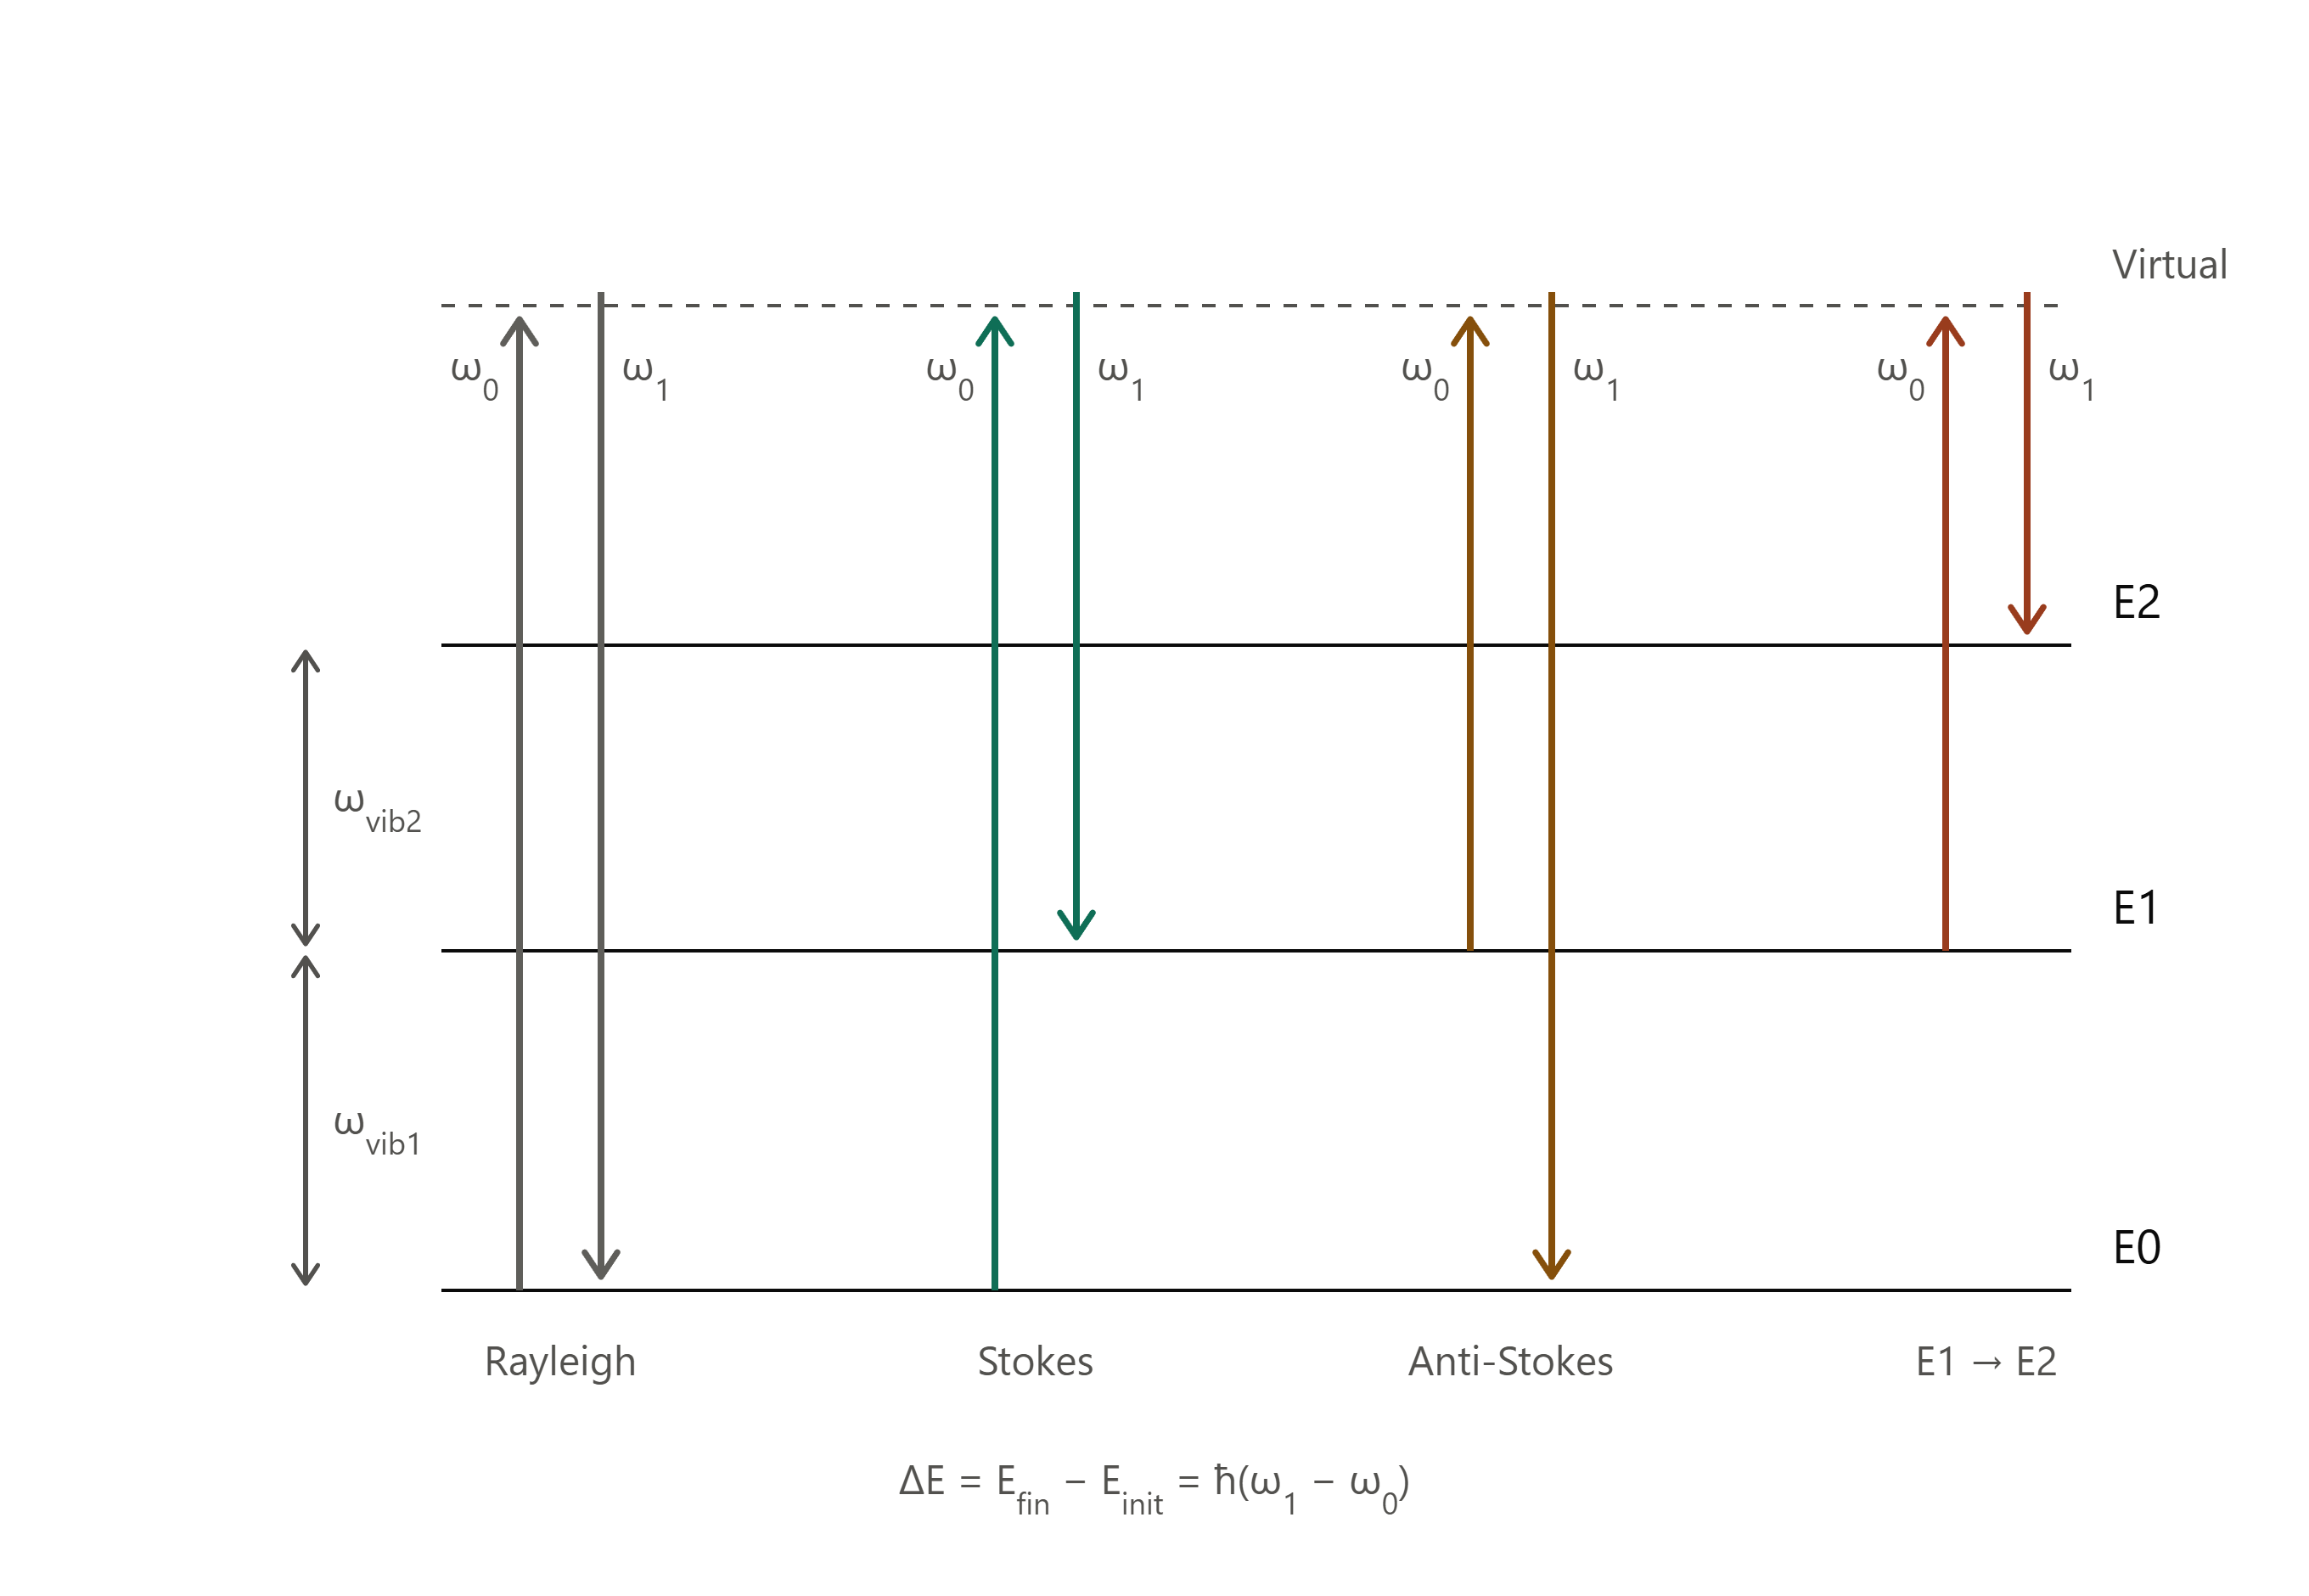
\includegraphics[width=\linewidth]{images/rayleigh_raman_energy_diagram.png}
    \caption{\footnotesize Diagram of energy model of the molecule-photon system.}
    \label{fig:energy_diagram}
\end{figure}

To understand the phenomenon let's consider a model of the energy of the system. Let's consider a very simple system with only one molecule and one photon. In figure \ref{fig:energy_diagram} we can see how the energy is transfered between the molecule and the photon. We know that energy states of molecules are discrete \cite{steinfeld2012molecules}, therefore changes in energy level of the molecule can only happen at precise quantities corresponding to the difference in energy levels. In the case of Rayleigh scattering, the molecular energy $E_{init} = E_{fin}$, and the incident and scattered photons have the same frequency, $\omega_s = \omega_1$. In the case of Raman scattering the molecular energy changes by $\Delta E = E_{fin}-E_{init} = \hbar ( \omega_1 - \omega_s)$, which is positive for Stokes scattering ($\omega_s < \omega_1$, the molecule gains energy) and negative for anti-Stokes scattering ($\omega_s > \omega_1$). Note that in all cases, the total energy of the photon-molecule system is preserved throughout this interaction.

Other types of light scattering exists and do happen in the course of performing Raman Spectroscopy. For example, at high incident intensities a molecule can scatter two photons at once, producing weak bands near $2\omega_1 \pm \omega_M$. This phenomenon is called hyper-Raman scattering. Another important phenomenon that interacts with the Raman signal is fluorescence, which manifests across larger band regions. We will address those issues when we deal with processing the signal. For illustration purposes, Figure \ref{fig:raw_spectrum} represents one raman spectrum from our dataset of Raman spectra of glioma biopsies.

\begin{figure}[h]
    \centering
    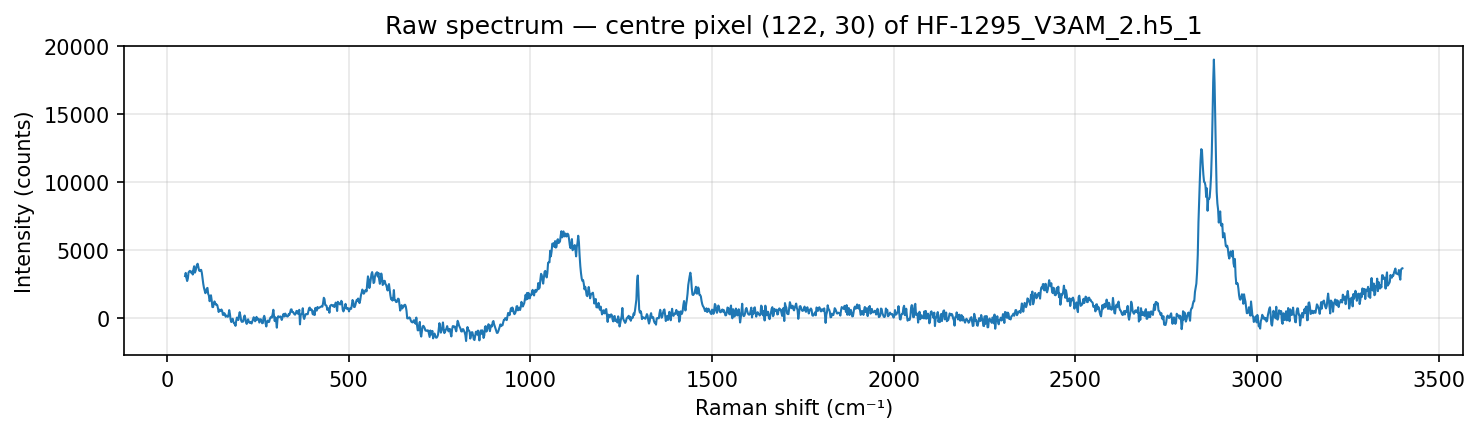
\includegraphics[width=\linewidth]{images/raw_spectrum_HF-1295_V3AM_2.h5_1.png}
    \caption{\footnotesize One raw spectrum of a sample in our dataset.}
    \label{fig:raw_spectrum}
\end{figure}

\section{Raman Spectroscopy in Medical Diagnosis}
\label{sec:rs_medical}
Many studies have been performed with RS in Medical Diagnosis, especially in oncology for tumor detection \cite{stupak2025raman,Auner2018}. However, given the high variability of protocols of using RS, and for lack of any standard protocol, results vary across study and are difficult to compare. Some examples of Raman protocols or techniques are: raw sample, frozen section, Surface Enhanced Raman Spectroscopy, Tip Enhanced Raman Spectroscopy, Resonance Raman Scattering, Surface Enhanced Resonance Raman Scattering, Spatially offset Raman Spectroscopy, Transmission Raman Spectroscopy, Coherent Anti-Stokes Raman Scattering, and Stimulated Raman Scattering \cite{Auner2018}.

RS produces raw spectra that are difficult or even impossible to interpret directly, therefore the standard approach in RS is to apply Machine Learning (ML) tools to map spectra to labels, as mapping the Raman spectrum to a chemical mixture of components is unfeasible, and often times impossible, especially for biological samples 
\cite{Boateng2025ramanmix}. This approach poses some difficulties in adoption of the method in medicine, as the models may not always be easily interpretable. However, given the high number of studies with promising results, it is possible that RS will be adopted in medicine in some form.

\TODO{A paragraph on the state of the ML side of the field, drawing on Sineesh and Kamsali \cite{sineesh2026raman}, who benchmark deep learning models for RS across open-source datasets and report four problems that recur regardless of application domain: (i) datasets are small; (ii) synthetic data is used extensively, but with unclear benefit in real-world application; (iii) there are few benchmarks, and deep models are seldom compared against classical ML or computer-vision baselines; and (iv) cross-paper performance comparison is difficult. State these in this general form here, since they frame every specific number quoted later: point (i) motivates the augmentation strategy of this work, point (ii) is precisely the question this thesis sets out to answer for glioma RS, point (iii) is why four downstream classifiers are evaluated rather than one, and point (iv) is why Table~\ref{tab:rs_brain_performance} reports validation schemes alongside accuracies. Note the pleasing symmetry: the field-wide critique in (ii) is what Chapter~\ref{sec:discussion} ends up confirming on this dataset.}



\subsection*{Reported performance in brain tumour applications}

\TODO{Write the prose around Table~\ref{tab:rs_brain_performance}; the numbers, cohorts and
validation schemes in it are taken from the three surveys and need no further checking. The
argument to build, in four moves:

(1) \emph{RS separates tumour from normal brain very well.} Reported accuracies cluster in
the 83--99\% range, and a meta-analysis over 1951 spectra puts glioma-vs-normal at 96\%
sensitivity / 99\% specificity. This is the result that motivates the whole field.

(2) \emph{Molecular classification is harder, and IDH status is the specific case this thesis
addresses.} Three groups report 87--89\% accuracy for IDH-mutant vs.\ IDH-wildtype, and
Livermore et al.\ report 91\% sensitivity / 95\% specificity. Note that the finer the
molecular distinction, the worse it gets: Galli et al.\ separate tumour from normal at
94--100\% but IDH-mutant oligodendroglioma from astrocytoma at only 81\%, and Zhou et al.\
fall from 99.6\% (glioma vs.\ normal) to 84.1\% (low- vs.\ high-grade) to 75.1\% overall on a
three-class problem. That degradation with granularity is the same pattern this work observes
between the binary task (Table~\ref{tab:binary_results}) and the six-class task
(Table~\ref{tab:sixclass_results}), and it is worth saying so explicitly.

(3) \emph{Cohorts are small.} The last column of Table~\ref{tab:rs_brain_performance} is the
one to dwell on: most studies work with fewer than 70 patients, several with fewer than 20.
The 58 slides used here are unremarkable for this literature -- which is the point, and the
motivation for the augmentation strategy of Section~\ref{sec:synthetic_rs}.

(4) \emph{Validation schemes differ enough to make the headline numbers hard to compare, and
this thesis's are conservative.} Most of these studies validate with leave-one-out or $k$-fold
cross-validation over \emph{spectra}, which places spectra from the same patient on both sides
of the split; a handful (Livermore et al., Riva et al.) use leave-one-patient-out. Under
patient-level validation the numbers fall: Riva et al.\ report 83\% for the comparatively easy
tumour-vs-normal task using random forests and gradient boosting -- the same model families
used here. Reading the $\sim$74\% of Table~\ref{tab:binary_results} against the 87--89\% IDH
figures without noting this difference would be misleading, and the honest comparison is the
one against Riva et al.\ and Livermore et al.

Be careful with attribution: these are three surveys, and Table~\ref{tab:rs_brain_performance}
credits the primary studies by name. If you want to cite the primary work directly rather
than the surveys, the DOIs are in the surveys' reference lists; as written, the table cites
the surveys, which is defensible for a background section.}

\begin{table}[htp]
\centering
\scriptsize
\caption{Reported performance of Raman spectroscopy in brain tumour applications, as collated
by three recent surveys \cite{hollon2021raman, murugappan2023raman, stupak2025raman}.
Grouped by task. Accuracy (Acc.), sensitivity (Sens.) and specificity (Spec.) in per cent;
a dash marks a figure the surveys do not report.}
\label{tab:rs_brain_performance}
\begin{tabular}{@{}p{3.3cm}p{3.1cm}p{2.2cm}>{\centering\arraybackslash}p{1.3cm}>{\centering\arraybackslash}p{1.2cm}>{\centering\arraybackslash}p{1.2cm}@{}}
\toprule
\emph{Study} & \emph{Cohort} & \emph{Validation} & \emph{Acc.} & \emph{Sens.} & \emph{Spec.}\\
\midrule
\multicolumn{6}{l}{\emph{Molecular / genetic classification}}\\
\midrule
Uckermann et al. & 36 froz. sect. & 5 bands, Mahal. & $89$ & -- & --\\
Sciortino et al. & fresh, post-resection & -- & $87$ & -- & --\\
Livermore et al. (IDH only) & 62 patients & LOPOCV & -- & $91$ & $95$\\
Livermore et al. (3 subtypes) & 62 patients & LOPOCV & -- & $79$--$94$ & $90$--$100$\\
Galli et al. (IDH-mut subtypes vs.\ astro) & 209 samples & PCA & $81$ & -- & --\\
\midrule
\multicolumn{6}{l}{\emph{Tumour vs.\ normal brain}}\\
\midrule
Zhang et al. (meta-analysis) & 1951 spectra & -- & -- & $96$ & $99$\\
Zhou et al. (VRRS) & -- & CV & $99.6$ & $100$ & $96.3$\\
Kalkanis et al. & frozen sections & -- & $97.8$ & -- & --\\
Iturrioz et al. & 4 patients & PCA-LDA & $92.5$ & -- & --\\
Jermyn et al. (\emph{in vivo}) & 17 pat., 161 spectra & LOOCV & $92$ & $93$ & $91$\\
Li et al. (KDE augment.) & 205 gl. / 37 norm. & -- & $91.67$ & $91.67$ & $91.67$\\
Riva et al. & 63 samples, 3450 spectra & LOPOCV, RF/GB & $83$ & -- & --\\
\midrule
\multicolumn{6}{l}{\emph{Grading}}\\
\midrule
Galli et al. (per subtype) & 209 samples & PCA & $86$--$100$ & -- & --\\
Zhou et al. (low vs.\,\ high grade) & -- & CV & $84.1$ & $96.3$ & $53.7$\\
Zhou et al. (normal / LGG / malignant) & -- & CV & $75.1$ & -- & --\\
Auner et al. (paediatric) & 64 samp., 28 pat. & PCA-DFA & $88.9$--$95.1$ & -- & --\\
\midrule
\multicolumn{6}{l}{\emph{Stimulated Raman histology (imaging, for context)}}\\
\midrule
Hollon et al. (SRH + CNN) & 278 patients & prosp. trial & $94.6$ & -- & --\\
Hollon et al. (H\&E comparator) & 278 patients & prosp. trial & $93.9$ & -- & --\\
Orringer et al. (SRH vs.\ H\&E) & 101 patients & $\kappa > 0.89$ & $>90$ & -- & --\\
\bottomrule
\end{tabular}
\small{LOOCV: leave-one-out cross-validation. LOPOCV: leave-one-patient-out cross-validation.
RF: random forest. GB: gradient boosting. VRRS: visible resonance Raman spectroscopy.
KDE: kernel density estimation. Note that only the LOPOCV entries guarantee that spectra from
one patient do not appear on both sides of the split; the remaining entries validate over
spectra, and their figures are correspondingly optimistic as estimates of performance on an
unseen patient.}
\end{table}

\subsection*{The study this dataset comes from}

\TODO{One or two paragraphs on Lita et al.\ \cite{apollonov2024raman}. This study is currently
mentioned only in passing in Chapter~\ref{sec:results}'s methodology, yet it supplies the
dataset, the labels, and the cross-validation design this work replicates -- it deserves to be
introduced properly here. Cover: what they set out to show (metabolic differences between
IDH-mutant and IDH-wildtype glioma detectable by RS), their preprocessing and tissue-selection
approach (PCA followed by DBSCAN over all spectra, which Section~\ref{sec:preprocessing_steps}
departs from and should justify departing from), the classifier they used (the RF+SVM
combination that appears here as one of the four downstream models), and the results they
reported. Then state plainly what this thesis adds on top: the generative augmentation, the
slide-level bootstrap, and the CbR inference strategy.}

\TODO{Optional but valuable: expand the existing paragraph on protocol heterogeneity. It
currently lists ten Raman variants in a single sentence and then asserts that results are hard
to compare. Say concretely why -- different excitation wavelengths, integration times,
normalisation choices and baseline-correction methods change the recorded spectrum, so a model
trained on one instrument's output does not transfer. This is the same instrument-variability
argument the introduction makes, and it motivates the augmentation strategy of this work.}


\section{Glioma Grading and Molecular Classification}
\label{sec:glioma_grading}

\TODO{This section does not yet exist and is the largest gap in this chapter. The thesis
classifies spectra into LGm1--LGm6 and into IDH-mutant vs.\ IDH-wildtype, but nowhere explains
where those categories come from or why they matter -- the labels are introduced in
Section~\ref{sec:data_collection} as a fait accompli. A reader should not have to take the
target variable on faith. Cover, in roughly this order:

(1) \emph{Clinical grading.} How gliomas are graded histopathologically, and the shift in the
WHO classification towards molecular rather than purely morphological criteria. Already cited
in the introduction: \texttt{whitfield2022classificationgliomas}. Note the turnaround time of
histopathology, since the case for RS in the introduction rests on it.

(2) \emph{IDH status.} What a mutation in isocitrate dehydrogenase does metabolically, why it
defines a prognostically distinct disease, and -- the point that matters here -- why the
resulting metabolic shift is large enough to leave a Raman signature. This is the biological
justification for the binary task being the easier of the two, an asymmetry the results
consistently show.

(3) \emph{The LGm methylation clusters.} Where LGm1--LGm6 come from: the pan-glioma DNA
methylation clustering of Ceccarelli et al.\ \cite{Ceccarelli2016}. State how the six clusters
map onto IDH status (LGm1--LGm3 mutant, LGm4--LGm6 wildtype), which is the grouping used
throughout this work. Then make the point that governs the 6-class results: methylation
subtypes are epigenetic distinctions, several steps removed from the molecular composition a
Raman spectrum measures, so there is no guarantee they are spectrally separable at all. The
~30\% 6-class accuracy in Section~\ref{sec:results_6class} is better read against that
expectation than against the binary result.

(4) \emph{Class imbalance as a clinical fact.} LGm1 and LGm6 are rare, which is why
Table~\ref{tab:dataset} is so uneven and why the cross-validation design of
Section~\ref{sec:cv_design} cannot be a clean partition. Worth stating here so that design
choice reads as forced rather than arbitrary.}

\section{Synthetic data for Raman Spectroscopy}
\label{sec:synthetic_rs}
Data augmentation is a comon technique used especially for Deep Learning (DL) models. In the context of RS, classic data augmentation techniques include (i) spectral shift, simulating instrument calibration drift, (ii) linear interpolation of spectra of the same class, or Synthetic Minority Over-sampling Technique (SMOTE), (iii) peak intensity perturbations \cite{zhao2024raman}.

A better approach involves learning the data distribution and constructing a generator of synthetic data. 

Evaluating such a data generator can be difficult, as we would like a quantitative measure of the data generator. Since a quantitative measure on the data itself may not be relevant for a particular task, the methodology of Train Real/Test Real vs. Train Synthetic/Test real was proposed \cite{esteban2017real}, where one trains a classifier on a real data train set, tests on a real data test set; the synthetic data generator is modeled on the train set, such that there is no data leakege from the test set via the generator. The same classifiers are then trained on synthetic data only, and tested on the same real data test set. This setup allows for quantitative measurements of the generator, as the training dataset can be compared against the synthetic data set. Any metric can be compared between the two models, such as accuracy, precision, recall, sensitivity, specificity.

A study of particular interest regarding synthetic data augmentation for RS in medical context was performed by Zhao et al. \cite{zhao2024raman} on in vivo skin cancer classification. They used a dataset of 731 spectra from 644 patients with 340 samples corresponding to cancerous and 391 corresponding to benign samples. They trained a 1D Generative Adversarial Network (GAN) on this data set and reported consistent improvements in accuracy in the range of 2-4\% across all classification models. Their findings suggest that deep generative data augmentation can help improve classification models.

\subsection*{Learned generative models for spectra}

\TODO{Half a page. The current text says only that "a better approach involves learning the
data distribution and constructing a generator" and then jumps straight to a single GAN study.
Fill in the families and what distinguishes them:
(i) GANs -- adversarial training, strong sample fidelity, but unstable to train and prone to
mode collapse, which is the failure mode this thesis observes in a VAE guise (the narrow
$\sigma$ envelope of Figure~\ref{fig:mean_std_spectra});
(ii) VAEs -- explicit likelihood bound, stable training, an interpretable latent space, at the
cost of blurrier / lower-variance samples. State plainly that this is the trade-off motivating
the choice made in this work, and forward-reference Section~\ref{sec:cvae};
(iii) diffusion models -- currently named in the future-work paragraph of
Chapter~\ref{sec:discussion} without ever having been introduced, which should be fixed here
even if only in two sentences.
Directly relevant entries already in the bibliography and uncited: \texttt{Gebran2025}
(conditional VAEs generating stellar spectra -- the closest published analogue to what this
work does, a CVAE generating 1-D spectra) and \texttt{Kavran2022} ($\beta$-VAE augmentation
for time-series classification, which is the same architecture class applied to the same kind
of sequential signal).}

\subsection*{Evaluating a generator}

\TODO{Extend the existing TS/TR paragraph, which covers the protocol but not what a generator
can fail at. The standard framing is three-way and worth stating explicitly, because this
thesis's results separate along exactly these axes:
(i) \emph{fidelity} -- are samples individually realistic? Here: yes, the mean spectra match
closely (Figure~\ref{fig:mean_std_spectra});
(ii) \emph{diversity} -- do samples cover the real distribution's spread? Here: no, and this
is the central negative finding;
(iii) \emph{privacy} -- do samples memorise training data? Relevant to the clinical
data-sharing motivation and worth a sentence even though this thesis does not measure it.
Uncited entry available: \texttt{jordon2022synthetic}. Note that a generator can score well on
a TS/TR classifier metric while failing (ii) badly, which is precisely the pattern in
Table~\ref{tab:binary_results} -- RF reaches 0.669 under TS/TR from a distribution far
narrower than the real one.}

\chapter{Theoretical Background}
\label{ch:theory}

This chapter provides the mathematical background for the methods used in this work. The
techniques are presented in the order in which the methodology applies them: first the
matrix factorization and clustering tools used to separate tumor spectra from background
(Sections~\ref{sec:nmf} and~\ref{sec:gmm}), then the neural network theory underlying the
generative model (Sections~\ref{sec:deep_learning} and~\ref{sec:cvae}), then the downstream
classifiers evaluated in Chapter~\ref{sec:results} (Section~\ref{sec:classifiers}), and
finally the embedding and statistical tools used to analyse the results
(Sections~\ref{sec:embeddings} and~\ref{sec:airpls_bootstrap}).


\section{Non-Negative Matrix Factorization}
\label{sec:nmf}

We will present here the problem of Non-Negative Matrix Factorization (NMF) with an emphasis on hyperspectral decomposition applications. This is a generic optimization problem with many applications and various theoretical formulations can be found, but we will formulate the problem in our context, as presented by Gillies \cite{Gillis2017,Gillis2020}.

The NMF can be formulated as follows: given a non-negative matrix $M \in \mathbb{R_+^{m \times n}}$, a factorization rank $r$, and a distance measure $D(\cdot,\cdot)$ find two non-negative matrices $W \in \mathbb{R}_+^{m \times r}$ and $H \in \mathbb{R}_+^{r \times n}$ such that $D(M,WH)$ is minimized, i.e. solve:
$$ \min_{W \in \mathbb{R}_+^{m \times r}, H \in \mathbb{R}_+^{r \times n}} D(M,WH)$$

In practice, we will consider the distance $D$ to be the Frobenius norm of the error matrix $M-WH$, hence the problem can be writen:

$$ \min_{W \in \mathbb{R}_+^{m \times r}, H \in \mathbb{R}_+^{r \times n}} \norm{M-WH}_F^2$$

This is the most natural and common choice as it corresponds to the assumption of i.i.d. Gaussian noise and it leads to a smooth optimization problem which is easy to solve \cite{Gillis2020}

There are many variants of NMF, for example the factorization can be solved exactly, in which case the problem is called Exact NMF, but in most applications we are only interested in an approximate solution. Also, for most solutions, additional constraints can be imposed.

The non-negativity constraints lead to natural physical interpretations of the terms of the factorization. The intuition is that spectral signatures are additive combinations of spectral signatures of the combining elements. For example, in our setting of biological samples, the spectral signature of a probe could be a linear combination of spectral signatures of lipids, proteins, phenilalanine, DNA C-H molecules, etc. This NMF factorization is called endmember unmixing, or more precisely, blind endmember unmixing, where individual components are called endmembers. Due to the additive nature of the signal acquisition process, where Raman bands appear where there is a certain molecule that has an absorbtion energy band of a specific energy level, this formulation of the NMF is well suited for the physical process involved.

\subsection*{Sparsity of factorization}

Non-negativity constraints are linear inequality constraints that naturally enforce sparsity, or solutions that contain lots of zeros. This derives from the first order optimality conditions (Karush-Kuhn-Tucker) of an optimization problem with such constraints \cite{Kuhn1951,Gillis2020}:

$$ \min_{x \in \mathbf{R^n}} f(x) \text{such that} x \ge 0 $$
giving the conditions:
$$ x \ge 0, \nabla f(x) \ge 0, \text{and} x_i(\nabla f(x))_i=0 \text{for all i.}$$

This enforces $x_i = 0$ if $(\nabla f(x))_i > 0$, which leads to sparse solutions.

\subsection*{Solution and Convergence}
Many algorithms have been developed for solving the NMF problem \cite{ChihJenLin2007,Xu2016,Lee2000}. We present here a simple solution by Daniel D. Lee and H. Sebastian Seung \cite{Lee2000}.

\begin{theorem}
    The distance $\norm{M-WH}_F^2$ is nonincreasing under the update rules
    $$ H_{a \mu} \leftarrow H_{a \mu} \frac{(W^T M)_{a \mu}}{(W^T W H)_{a \mu}} \qquad
    W_{i a} \leftarrow W_{i a} \frac{(M H^T)_{i a}}{(W H H^T)_{i a}}$$
    This distance is invariant under these updates iff $W$ and $H$ are at a stationary point.
\end{theorem}

The proof of convergence can be found in full in D.D. Lee's article. We can see that the updates alternate, hence it resembles the Expectatio-Maximization algorithm. \cite{Lee2000}.

In our analysis we used the scikit-learn implementation of the NMF \cite{sklearn2011,Cichocki2009}.

\section{Gaussian Mixture Model}
\label{sec:gmm}

The Gaussian Mixture Model (GMM) is a widely used tool that assigns soft labels to a set of data points. We can consider it a soft clustering technique, where we define a hard clustering as a partition of the set of points and a soft clustering a labeling of the points with a probability distribution over the number of clusters.
We present here a short description of the method as described by C.H. Bishop in "Pattern Recognition and Machine Learning", Chapter 9 \cite{bishop2006pattern}.

The Gaussian Mixture can be defined as a weighted sum of Gaussian distributions:

$$ p(\mathbf{x}) = \sum_{k=1}^{K}\pi_k \mathcal{N}(\mathbf{x} | \mu_k, \Sigma_k) $$

where $\mathbf{x}$ is the data set $\mathbf{x} = \{x_1, x_2, \dots x_N\}$. In order to assign points to clusters, we will assume there exists this assignment as a latent variable. We will denote this latent variariable with $\mathbf{z}$, as unit vectors of $\mathbb{R}^K$. We can now define the joint distribution $\mathbb{P}(\mathbf{x},\mathbf{z})$, the marginal distribution $\mathbb{P}(\mathbf{z})$, the conditional distribution $\mathbb{P}(\mathbf{x}|\mathbf{z})$. The marginal distribution over $\mathbf{z}$ is:
$$\mathbb{P}(z_k = 1) = \pi_k$$
where the parameters $\{\pi_k\}$ form a probability distribution, so they must satisfy the constraints:
$$0 \le \pi_k \le 1 \quad \sum_{k=1}^{K}\pi_k = 1$$
Because $z_k \in \{0,1\}$, we can write:
$$\mathbb{P}(\mathbf{z}) = \prod_{k=1}^K \pi_k^{z_k}$$
We make the assumption that the conditional distribution of x given z is a Gaussian:
$$\mathbb{P}(\mathbf{x}|z_k = 1) = \mathcal{N}(\mathbf{x} | \mu_k, \Sigma_k)$$

By summing over all states of z we obtain the marginal distribution of x:

$$ \mathbb{P}(x) = \sum_{\mathbf{z}} \mathbf{P}(\mathbf{z})\mathbf{P}(\mathbf{x}|\mathbf{z}) = \sum_{k=1}^{K} \pi_k \mathcal{N(\mathbf{x}|\mu_k, \Sigma_k)}$$

Of particular interest is also the conditional probability of $\mathbf{z}$ given $\mathbf{x}$. We will use the following notation:
$$\gamma(z_k) := \mathbb{P}(z_k=1|x) = \frac{\mathbb{P}(z_k = 1) \mathbb{P}(\mathbf{x}|z_k = 1) }{\sum_{j=1}^{K} \mathbb{P}(z_j = 1) \mathbb{P}(\mathbf{x}|z_j = 1} = \frac{\pi_k \mathcal{N}(\mathbf{x}|\mu_k, \Sigma_k)}{\sum_{j=1}^{K} \pi_j \mathcal{N}(\mathbf{x}|\mu_j, \Sigma_j)}$$

We can now view $\pi_k$ as the prior probability and $\gamma(z_k)$ as the posterior after observing $x$.

With $\mathbf{x}$ as our dataset, the log of the likelihood can be written as:
$$ \ln \mathbb{P}(\mathbf{x}|\pi,\mu,\Sigma) = \sum_{n=1}^{N} \ln \left\{\sum_{k=1}^{K} \pi_k \mathcal{N}(\mathbf{x}_n|\mu_k,\Sigma_k)\right\} $$

To find the maximum of this function, we set the derivatives with respect to $\mu_k$ to 0 and we obtain:
$$ \mu_k = \frac{1}{N_k} \sum_{n=1}^{N}\gamma(z_{nk})\mathbf{x}_n $$
where
$$ N_k = \sum_{n=1}^{N} \gamma(z_{nk}) $$

Next we set the derivatives with respect to $\Sigma_k$ to zero and we obtain:

$$ \Sigma_k = \frac{1}{N_k} \sum_{n=1}^{N}\gamma(z_{nk})(\mathbf{x}_n - \mu_k)(\mathbf{x}_n - \mu_k)^T $$

In order to find the $\pi_k$ coeficients, we take into account the probability constraints over $\pi_k$ and we maximize:
$$ \ln \mathbb{P}(\mathbf{x}|\pi, \mu, \Sigma) + \lambda \left(\sum_{k=1}^{K} \pi_k - 1 \right)$$
and we obtain
$$ \pi_k = \frac{N_k}{N} $$

\subsection*{The Expectation Maximization algorithm}

We cannot find a direct solution to the GMM problem, but we can devise an iterative algorithm by alternating between the cluster assignments and the parameters of the gaussians. The algorithm is called Expectation Maximization (EM):



\begin{algorithm}
\caption{The EM Algorithm}
\begin{algorithmic}[1] 
    \State \textbf{Initialize:} Randomly initialize $\mu_k$, $\Sigma_k$, $\pi_k$ 

    
    \While{not converged} 
        
        \State \textbf{E step: evaluate the clustering}
        \vspace{1.5ex} % Spacing before the E-step formula
        \Statex \hspace{\algorithmicindent} $\displaystyle \gamma(z_{nk}) = \frac{\pi_k \mathcal{N}(\mathbf{x}_n|\mu_k,\Sigma_k)}{\sum_{j=1}^{K} \pi_j \mathcal{N}(\mathbf{x}_n|\mu_j,\Sigma_j)}$
        \vspace{2.5ex} % Spacing after the E-step formula
        
        \State \textbf{M step: estimate parameters using the current clustering}
        \vspace{1.5ex} % Spacing before the M-step aligned formulas
        \Statex \hspace{\algorithmicindent} $\begin{aligned}
            \mu_k^{\text{new}} &= \frac{1}{N_k} \sum_{n=1}^{N} \gamma(z_{nk}) \mathbf{x}_n \\[1.5ex]
            \Sigma_k^{\text{new}} &= \frac{1}{N_k} \sum_{n=1}^{N} \gamma (z_{nk})(\mathbf{x}_n - \mu_k^{\text{new}})(\mathbf{x}_n - \mu_k^{\text{new}})^T \\[1.5ex]
            \pi_k^\text{new} &= \frac{N_k}{N} \quad \text{where} \quad N_k = \sum_{n=1}^{N} \gamma(z_{nk})
        \end{aligned}$
        \vspace{2.5ex} % Spacing after the M-step formulas
        
        \State \textbf{Evaluate the log likelihood for the entire dataset} 
        \vspace{1.5ex} % Spacing before the log-likelihood formula
        \Statex \hspace{\algorithmicindent} $\displaystyle \ln \mathbb{P}(\mathbf{x}|\mu, \Sigma, \pi) = \sum_{n=1}^{N} \ln \left( \sum_{k=1}^{K} \pi_k \mathcal{N}(\mathbf{x}_n| \mu_k, \Sigma_k) \right)$
        \vspace{2ex} % Spacing before the loop ends

    \EndWhile
\end{algorithmic}
\end{algorithm}

Note that this is an iterative algorithm and it converges to a local solution. While this works in practice most of the time, there exists the posibility that the solution is not optimal.

\section{Deep Learning}
\label{sec:deep_learning}

Research in Artificial Neural Networks, or Deep Learning has expanded significantly in the last decades, motivated by advances in computing power, development of software frameworks for easy implementation and testing, as well as theoretical results that offer some guarantees regarding the behaviour of Artificial Neural Networks. 

\subsection*{Early results: ANNs as Universal Function Approximators}
The first theoretical results were formulated in 1989, with Kurt Hornik et al. \cite{Hornik1989} prooving that a Neural Network with one hidden layer, with a squashing activation function can aproximate arbitrarily well any continuous function on a compact set, provided we let the number of neurons in the hidden layer grow arbitrarily large, and G. Cyabenko proving the Universal Approximator theorem for sigmoid activation functions \cite{Cybenko1989}.

\subsection*{Extending the Universal Function Approximation Theorem}
Other activation functions were tested, and as the requrements on the function were reduced to continuous, non linear, and differentiable almost everywhere, the function $X^+$ (0 if $x < 0$, $x$ otherwise), known in the Deep Learning comunity as the Rectified Linear Unit (ReLU) activation function became widespread.

The theorem of Universal Approximation was proved for the ReLU activation function as well under some particular geometries \cite{Hanin2019, Lu2017}. 

Other variants of the theorem relevant for our design are the ones regarding the convolution operation \cite{Zhou2020, Yarotsky2018}. This acts as a shared local operator replacing the full matrix multiplication .

We observe that there are many variants of the Universal Approximation Theorem, and many different proofs for various ANNs different geometries, activation function or other components like local operators.


\section{Conditional Variational Autoencoder}
\label{sec:cvae}

The generative model used in this work is a Conditional Variational Autoencoder (CVAE). This
section develops it in three steps: the variational autoencoder as a latent variable model
\cite{kingma2014vae}, the Evidence Lower Bound that makes it trainable, and the conditioning
mechanism that turns it into a class-conditional generator \cite{sohn2015cvae}. The
architecture and the training objective actually used are given in
Section~\ref{sec:cvae_architecture}.

\subsection*{The latent variable model}

We assume the observed spectra $x \in \mathbb{R}^{N_\lambda}$ are generated by a two-stage
process: a latent variable $z \in \mathbb{R}^{d}$ is drawn from a prior $p(z)$, and the
spectrum is then drawn from a conditional distribution $p_\theta(x|z)$ parameterised by a
neural network with parameters $\theta$. The marginal likelihood of a spectrum is therefore
\begin{equation}
p_\theta(x) = \int p_\theta(x|z)\, p(z) \, dz .
\label{eq:marginal_likelihood}
\end{equation}

Maximising \eqref{eq:marginal_likelihood} directly is intractable: the integral runs over the
whole $d$-dimensional latent space, and $p_\theta(x|z)$ is a neural network, so no closed form
exists. The same intractability affects the true posterior
\begin{equation}
p_\theta(z|x) = \frac{p_\theta(x|z)\,p(z)}{p_\theta(x)},
\label{eq:true_posterior}
\end{equation}
whose denominator is exactly the intractable quantity \eqref{eq:marginal_likelihood}.

The variational approach sidesteps this by introducing a second neural network, the
\emph{encoder} $q_\phi(z|x)$ with parameters $\phi$, which approximates the true posterior
$p_\theta(z|x)$. Rezende et al.\ \cite{rezende2014stochastic} show that parameterising the
mean and variance of a Gaussian by neural networks in this way is sufficient to approximate
complex posterior densities, which justifies the Gaussian choice made below.

\TODO{One paragraph of intuition here: the encoder compresses a spectrum into a
low-dimensional code and the decoder reconstructs it, but unlike a plain autoencoder both
maps are distributions rather than points. Say why a distribution is what makes sampling
possible later.}

\subsection*{The Kullback--Leibler divergence}

For two distributions $q$ and $p$ over the same space, the Kullback--Leibler divergence is
\begin{equation}
D_{KL}(q \| p) = \mathbb{E}_{q}\left[ \log \frac{q(z)}{p(z)} \right]
              = \int q(z) \log \frac{q(z)}{p(z)} \, dz .
\label{eq:kl_definition}
\end{equation}
It is non-negative, and zero if and only if $q = p$ almost everywhere. It is not symmetric, so
it is not a metric; $D_{KL}(q\|p)$ measures the cost of describing samples from $q$ using a
code built for $p$.

\subsection*{The Evidence Lower Bound}

Starting from the log marginal likelihood and introducing $q_\phi(z|x)$:
\begin{align}
\log p_\theta(x)
  &= \log \int p_\theta(x|z)\,p(z)\,dz
   = \log \int q_\phi(z|x) \frac{p_\theta(x|z)\,p(z)}{q_\phi(z|x)} \, dz \nonumber \\
  &= \log \mathbb{E}_{q_\phi(z|x)}\!\left[ \frac{p_\theta(x|z)\,p(z)}{q_\phi(z|x)} \right]
   \;\ge\; \mathbb{E}_{q_\phi(z|x)}\!\left[ \log \frac{p_\theta(x|z)\,p(z)}{q_\phi(z|x)} \right],
\label{eq:jensen}
\end{align}
where the inequality is Jensen's inequality applied to the concave function $\log$. Splitting
the logarithm gives the Evidence Lower Bound (ELBO):
\begin{equation}
\mathcal{L}_{\text{ELBO}}(\theta,\phi;x)
 = \underbrace{\mathbb{E}_{q_\phi(z|x)}\big[ \log p_\theta(x|z) \big]}_{\text{reconstruction}}
 - \underbrace{D_{KL}\big(q_\phi(z|x) \,\|\, p(z)\big)}_{\text{regularisation}} .
\label{eq:elbo}
\end{equation}

The gap between the bound and the true log-likelihood is itself a KL divergence,
\begin{equation}
\log p_\theta(x) - \mathcal{L}_{\text{ELBO}}(\theta,\phi;x)
 = D_{KL}\big(q_\phi(z|x) \,\|\, p_\theta(z|x)\big) \;\ge\; 0 ,
\label{eq:elbo_gap}
\end{equation}
so maximising the ELBO simultaneously raises a lower bound on the evidence and drives the
approximate posterior towards the true one.

\TODO{Two or three sentences reading equation \eqref{eq:elbo} back in words: the first term
rewards faithful reconstruction, the second penalises latent codes that stray from the prior,
and training balances the two. Connect this to the composite loss in
Section~\ref{sec:cvae_architecture}, where the reconstruction term is realised as MSE and
cosine loss and the KL term carries the weight $\beta$.}

\subsection*{The Gaussian case and the reparameterisation trick}

We take the prior to be a standard normal, $p(z) = \mathcal{N}(0, I)$, and the approximate
posterior to be a diagonal Gaussian whose parameters are produced by the encoder,
\begin{equation}
q_\phi(z|x) = \mathcal{N}\big(z \,;\, \mu_\phi(x), \, \operatorname{diag}(\sigma^2_\phi(x))\big).
\label{eq:gaussian_posterior}
\end{equation}
Under these choices the KL term of \eqref{eq:elbo} has the closed form used in
Section~\ref{sec:cvae_architecture}:
\begin{equation}
D_{KL}\big(q_\phi(z|x) \| p(z)\big)
 = \frac{1}{2} \sum_{i=1}^{d} \left( \mu_i^2 + \sigma_i^2 - \log(\sigma_i^2) - 1 \right).
\label{eq:kl_gaussian}
\end{equation}
In practice the encoder emits $\log(\sigma_i^2)$ rather than $\sigma_i$, which keeps the
variance positive without a constraint and is numerically better behaved.

The reconstruction term of \eqref{eq:elbo} is an expectation over $q_\phi(z|x)$, estimated in
training by sampling $z$. Sampling is not differentiable with respect to $\phi$, so the
gradient cannot be propagated back into the encoder. The \emph{reparameterisation trick}
\cite{kingma2014vae} resolves this by moving the randomness into a parameter-free variable:
\begin{equation}
z = \mu_\phi(x) + \sigma_\phi(x) \odot \epsilon,
\qquad \epsilon \sim \mathcal{N}(0, I),
\label{eq:reparameterisation}
\end{equation}
where $\odot$ is the elementwise product. The sample $z$ is now a deterministic, differentiable
function of $\mu_\phi(x)$ and $\sigma_\phi(x)$, and the gradient flows through it while the
stochasticity is confined to $\epsilon$.

\subsection*{Why the KL term turns the decoder into a generator}

\TODO{This subsection is the conceptual keystone of the thesis and deserves a careful
paragraph in your own words. The argument to make: to generate a new spectrum we sample
$z \sim \mathcal{N}(0,I)$ and pass it through the decoder, but this is only meaningful if the
decoder has actually been trained on inputs distributed that way. A plain autoencoder places
its codes wherever reconstruction is easiest, leaving regions of latent space the decoder has
never seen, so a prior sample from such a region decodes to noise. The KL term in
equation \eqref{eq:elbo} penalises exactly this: it pulls the aggregate distribution of
encoded spectra towards the prior, so that the region the decoder was trained on and the
region we sample from coincide. Then state the trade-off: raising $\beta$ tightens that match
at the cost of reconstruction fidelity \cite{higgins2017betavae}, and note that
Chapter~\ref{sec:discussion} finds the resulting synthetic spectra to have visibly narrower
variance than the real ones -- which is this trade-off made visible.}

\subsection*{Conditioning: from VAE to CVAE}

To control which class a generated spectrum belongs to, both encoder and decoder receive the
class label $y$ as an additional input \cite{sohn2015cvae}. The ELBO becomes
\begin{equation}
\mathcal{L}_{\text{ELBO}}(\theta,\phi;x,y)
 = \mathbb{E}_{q_\phi(z|x,y)}\big[ \log p_\theta(x|z,y) \big]
 - D_{KL}\big(q_\phi(z|x,y) \,\|\, p(z|y)\big),
\label{eq:celbo}
\end{equation}
and the prior is usually taken to be independent of the label, $p(z|y) = p(z) = \mathcal{N}(0,I)$,
so that a single latent space is shared across classes and the label alone selects the class.

Generation is then immediate: draw $z \sim \mathcal{N}(0, I)$, choose a one-hot label $y_c$,
and evaluate $\hat{x} = p_\theta(x | z, y_c)$. This is the sampling procedure used to build
the synthetic training sets of Chapter~\ref{sec:experimental_design}, and, run once per
candidate class, it is also the mechanism behind the Classification by Reconstruction strategy
of Section~\ref{sec:cbr}.

\TODO{Optional closing paragraph: note that conditioning the decoder does not by itself
guarantee class-discriminative latent codes, which is the motivation for the auxiliary
classification head described in Section~\ref{sec:cvae_architecture}. Related applications of
conditional VAEs to spectral and time-series data: \texttt{Gebran2025} (stellar spectra),
\texttt{Kavran2022} (beta-VAE augmentation for time series).}

\chapter{Methodology}
\label{ch:methodology}

This section describes the data workflow from preprocessing to evaluation and the tools we used at each step. We designed our workflow into four stages:
\begin{itemize}
    \item preprocessing and slide level data processing
    \item selection of valid spectra
    \item training models and synthetic data generation
    \item evaluation under the TS/TR and TSR/TR regimes against the baseline TR/TR
\end{itemize}

\section{Data Collection}
\label{sec:data_collection}

We analyzed the dataset of glioma RS biopsies collected for the study performed by Lita et al. \cite{apollonov2024raman}. The data acquizition protocol is described in detail in their study. The biological samples and the corresponding methylome labels were provided by Dr. Houtan Noushmehr; the samples were collected at the Hermelin Brain Tumor Center at Henry Ford Health System. The samples were anonymized and all the patients consented to have their acquired data used for research purposes.

The resulting dataset consists of approximately $270{,}000$ Raman spectra from 59 biopsy scans. One scan, \texttt{HF-1887\_via-t\_2\_1.h5\_3}, was excluded for data quality reasons, leaving the 58 scans used throughout this work; the exclusion is recorded in the \texttt{ignore\_samples} field of every experiment configuration. Each sample scan is a $(H_i,W_i,N_\lambda)$ tensor, with $H_i$ and $W_i$ the width and height of the slide $i$, in number of pixels, and $N_\lambda = 1738$ represents the number of spectral bands or spectral dimension, which is constant throught the dataset as all of the samples were processed with the same spectrometer.

The samples are labeled with LGm1 to LGm6, corresponding to 6 distinct methylation profiles. The labels (LGm1, LGm2, LGm3) are all classified as IDH-mutant tumour, while the labels (LGm4, LGm5, LGm6) are classified as IDH-wildtype. This coarser classification is very important, as it corresponds to a much higher physiological difference than the differences between methylation profiles. This allows us to formulate two problems, one of binary classification of tumour grade between mutant and wildtype and a more difficult problem of determining the methylation profile. The number of samples per class can be found in Table \ref{tab:dataset}

\begin{table}[h]
\centering
\caption{Number of slides and patients by methylation subtype, for the 58 slides retained for
analysis.}
\label{tab:dataset}
\begin{tabular}{llcccc}
\toprule
\textbf{Methylation} & \textbf{IDH Group} & \textbf{Slides} & \textbf{Group total} & \textbf{Patients} & \textbf{Group total} \\
\midrule
LGm1 & Mutant   & 5  &    & 5  & \\
LGm2 & Mutant   & 11 & 25 & 11 & 20 \\
LGm3 & Mutant   & 9  &    & 4  & \\
\midrule
LGm4 & Wildtype & 13 &    & 10 & \\
LGm5 & Wildtype & 15 & 33 & 11 & 25 \\
LGm6 & Wildtype & 5  &    & 4  & \\
\midrule
\multicolumn{2}{@{}l}{\textbf{Total}} & \textbf{58} & & \textbf{45} & \\
\bottomrule
\end{tabular}
\small{Slides outnumber patients because several patients contributed more than one tissue
section; the cross-validation scheme of Section~\ref{sec:cv_design} therefore splits at the
patient level. The excluded LGm2 slide is not counted here. The population-level subtype
distribution is compared against this composition in Table~\ref{tab:glioma_distribution}.}
\end{table}

\subsection{Cross Validation design}
\label{sec:cv_design}
For rigurous results, we want to implement a Cross Validation (CV) scheme. Standard CV divides the samples into N subsets of approximately equal size that form a partition of the dataset. Training is performed on N-1 subsets and testing on the subset left out of the training phase. In more complex settups where the classes are imbalanced, the CV split needs to be performed stratified by class to ensure that all classes are represented in each CV split. In cases where some classes are severely underrepresented, like the LGm1 and LGm6 classes, a standard CV split might be impossible to acheive. In our case, we aim to perform a 5 fold CV split at patient level. Out of the 5 samples of class LGm6, some belong to the same patient, which makes a standard CV split impossible. However, we can relax the requirements a bit without losing the rigour of data splitting. We can drop the requirement that the split forms a partition, but keep the train-test separated at patient level for all folds. This is the CV design used by Lita et al. The full detailed CV split can be found in the Appendix.

\section{Data Preprocessing}
\label{sec:preprocessing_steps}

An important first step in data processing is separating the useful signal from the noisy measurements. We would like to seprate the tumor spectra from the healthy tissue or non-tissue measurements. As each spectrum corresponds to a pixel on the biopsy slide, it is possible that some pixels do not contain tissue and that the laser probe hit the plate material. A lot of slides appear to have some spots where there is no tissue; the cluster assignment maps in Fig.\ \ref{fig:preprocessing_cluster_spectra}(a, c) show such regions as contiguous areas of weak signal at the slide margins. In the absence of a ground truth labeling, we must rely on unsupervised techniques. In previous studies various techniques have been proposed. For example in the study by Lita et al. on this dataset they proposed the use of PCA followed by DBSCAN on all spectra. We decided to take a more conservative approach and to make the decision per slide, and to visually inspect the clusterings to double check the results. The proposed annotation pipeline consists of the following steps:

\begin{figure}[h]
    \centering
    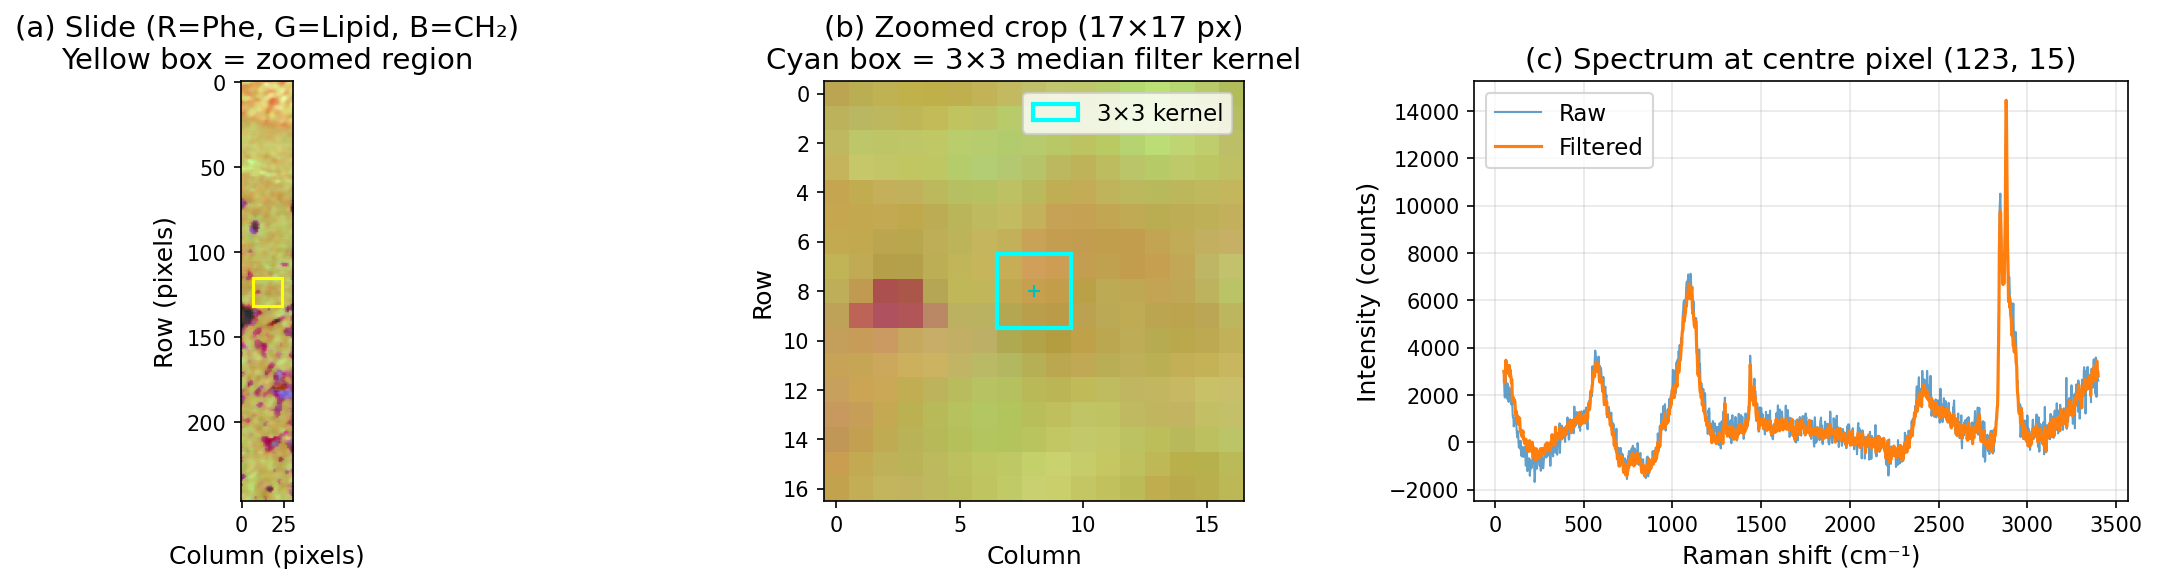
\includegraphics[width=\linewidth]{images/preprocessing_median_filter_illustration.png}
    \caption{\footnotesize (a) False coloring of a slide, with Red = Phenylalanine marker (990--1020 $\text{ cm}^{-1}$), Green = Lipids (2800--3000 $\text{ cm}^{-1}$), Blue = $CH_2$ deformations (1430--1460 $\text{ cm}^{-1}$). (b) Zoomed region for $3\times 3$ median kernel visualization. (c) Raw vs. Median filtered spectra.}
    \label{fig:preprocessing_median_filter_illustration}
\end{figure}

\begin{enumerate}
    \item \emph{Median filtering.} A $3 \times 3$ median kernel was applied on the spatial dimensions $(H,W)$ of each slide for denoising purposes, filtering out cosmic radiation and Gaussian noise (See Fig. \ref{fig:preprocessing_median_filter_illustration}). More specifically, given a position $(i,j)$, and a raw slide $S$ of size $(H,W,N_\lambda)$, let $S(i,j,l)$ be the value of the spectral band $l$ at position $(i,j)$. Then the median filtered spectral band $l$ at position $(i,j)$ is 
    $$ \text{median}(S(i,j,l)) = \text{median} \left( \left( S(\hat{i}, \hat{j}, l) \right)_{\hat{i}, \hat{j}} : \hat{i} \in \overline{i-1:i+1}, \hat{j} \in \overline{j-1:j+1} \right) $$

    \item \emph{Slide-wise normalization.} Each data tensor was normalized independently to the $[0,1]$ range to ensure numerical stability. We note that this means the entire tensor is divided by the maximum value of the tensor.

    \item \emph{Signal filtering.} We applied a simple signal quality filter by removing spectra with low intensity, setting a threshold of 0.6 on the maximum intensity of the spectrum. This step eliminates spectra that are likely dominated by noise or background, as they typically have low overall intensity. We plotted a histogram of the maximum intensity values across all spectra per slide and observed that most of the spectra have a maximum intensity close to 1, while a small subset of spectra was below the fixed threshold, hence considered low quality and removed from the dataset. Our threshold choice is rather conservative; from the maximum intensity histograms, it can be observed that a higher threshold can be selected (see Fig. \ref{fig:preprocessing_cluster_spectra} e, f).

    \item \emph{Spectral dimensionality reduction.} 

    Non-negative Matrix Factorization (NMF) \cite{NMF1999} was applied independently to each slide to obtain a lower-dimensional, non-negative representation of the spectra. NMF has previously been used in Raman spectroscopy for spectral unmixing and feature extraction \cite{NMF1999,nmf_oncology_2022, Alix2022}. We used an NMF with 100 components, as it offered sufficient reconstruction for the purpose of signal separation. 
    
    \item \emph{Gaussian Mixture Model (GMM).} A 3-component Gaussian Mixture Model (GMM) was fitted to the coefficients obtained in the previous step. We then visually inspected the clustering and selected the spectra corresponding to the components with the strongest signal. In cases where more than one cluster had similar quality spectra, and the clusters were not spatially separated in distinct regions, we selected all of them as valid spectra. This is why we refer to our pipeline as spatio-spectral as we visually analyze the clusters in both the spectral domain and the spatial domain.
    

\begin{figure}[h]
    \begin{minipage}[b]{\linewidth}
    \centering
    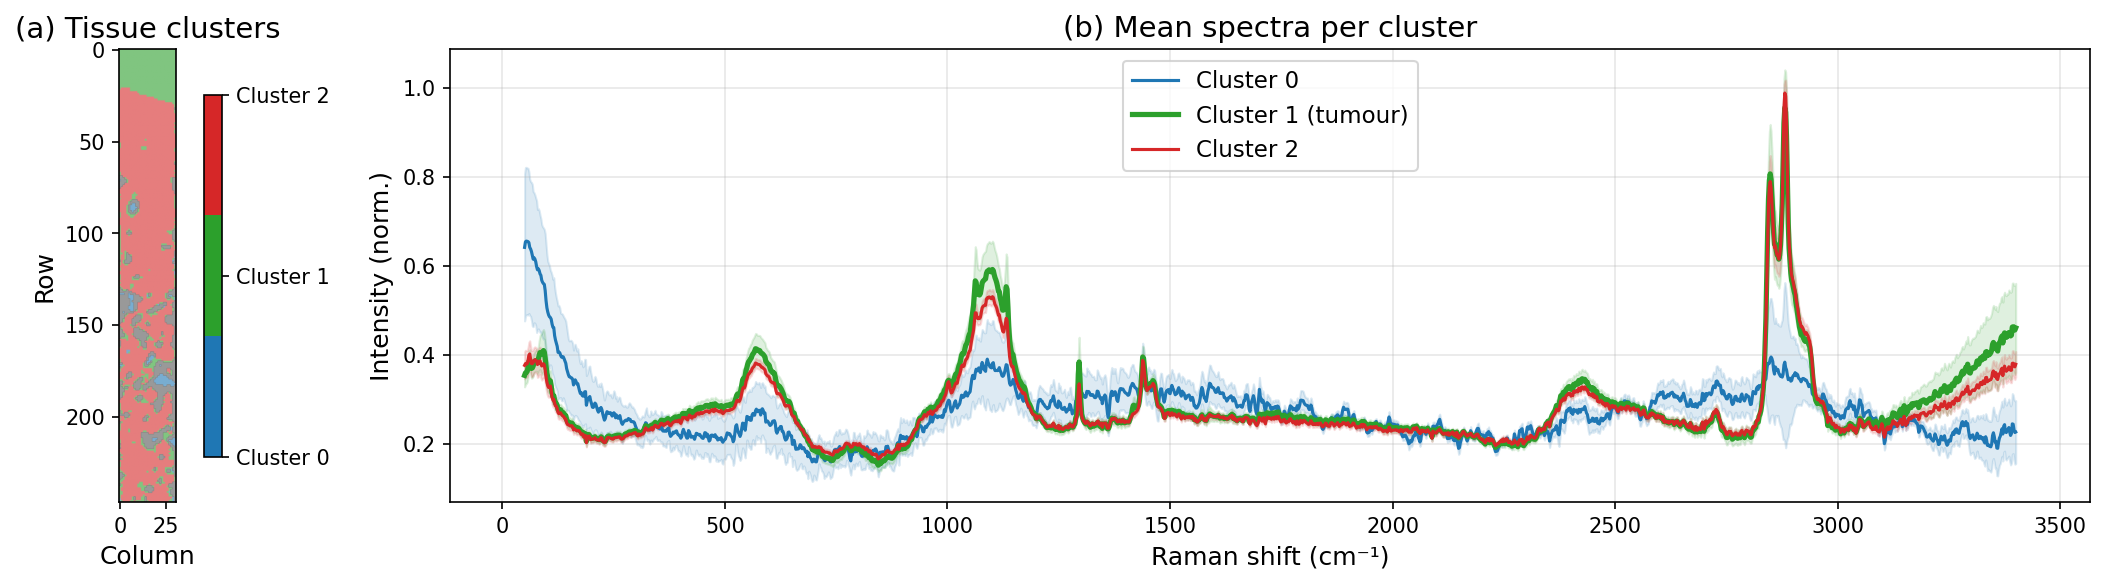
\includegraphics[width=\linewidth]{images/preprocessing_cluster_spectra.png} 
  \end{minipage}\\
  \begin{minipage}[b]{\linewidth}
    \centering
    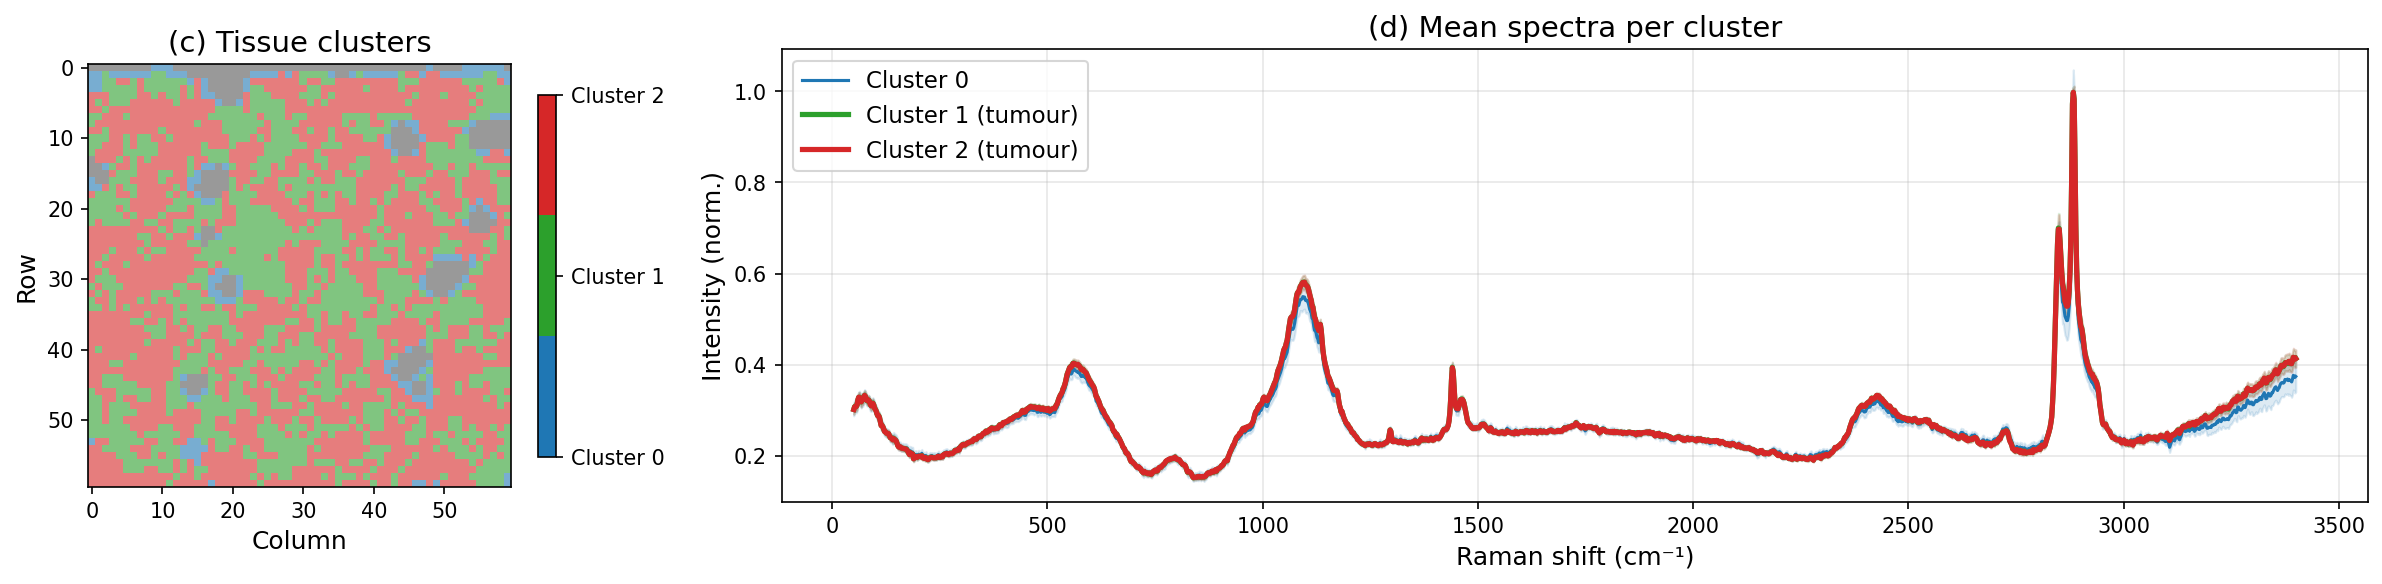
\includegraphics[width=\linewidth]{images/preprocessing_cluster_spectra_2.png} 
  \end{minipage}\\
  \begin{minipage}[b]{0.5\linewidth}
    \centering
    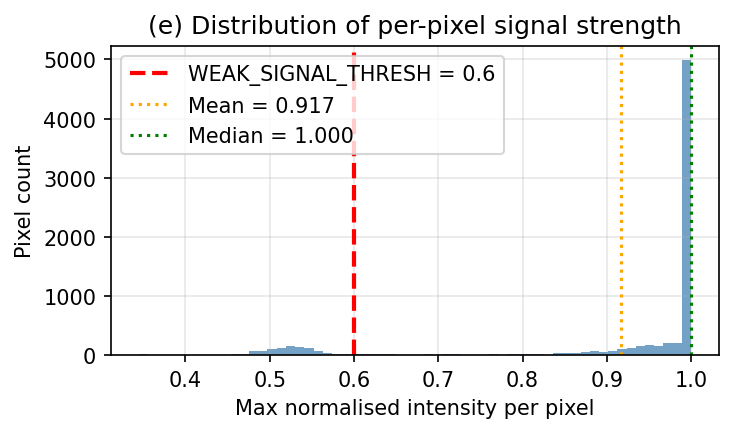
\includegraphics[width=\linewidth]{images/max_vals_distribution_img_0.png}
    \vspace{1ex}
  \end{minipage}%% 
  \begin{minipage}[b]{0.5\linewidth}
    \centering
    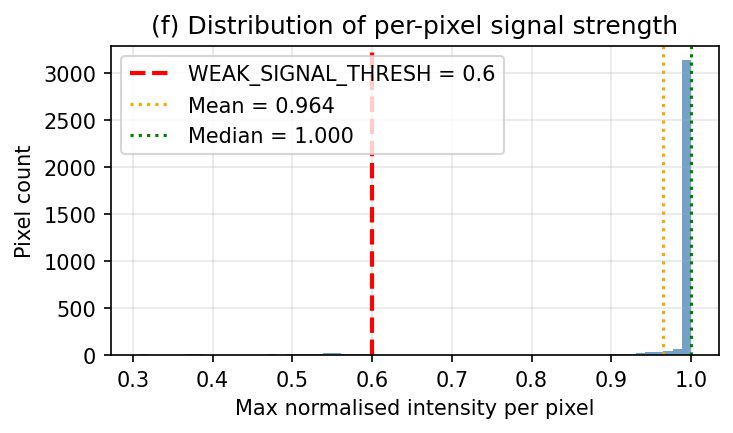
\includegraphics[width=\linewidth]{images/max_vals_distribution_img_5.png} 
    \vspace{1ex}
  \end{minipage}    
    \caption{\footnotesize Spectral clustering of two slides (top, middle). (a) Slide 1 cluster assignment; (b) Slide 1 Mean spectra per cluster: blue = weak signal cluster, discarded, red = medium intensity signal, discarded, green = strong signal, selected as tumor; (c) Slide 2 cluster assignment; (d) Slide 2 Mean spectra per cluster: red, green = strong tissue signal, selected as tumor, blue = weak signal, discarded; (e, f) Histograms of maximum intensity of spectra for the first and second slides, respectively.}
    \label{fig:preprocessing_cluster_spectra}
\end{figure}


    \item \emph{Per spectrum preprocessing.} For the spectra selected as relevant, we performed the following per spectrum processing steps: (i) [0, 1] normalization; (ii) airPLS with $\lambda=100$ and porder $p=1$; 
    

    \item \emph{Saving spectra.} We saved the processed spectra to an HDF5 file for further ML tasks. Note that we used NMF only for clustering, but the processing for saved spectra was $3 \times 3$ median filtering followed by airPLS baseline correction. We preferred to keep as much of the signal as possible, and also to keep the preprocessing simple and reproducible. The NMF reconstruction smothes the signal further, and we prefer to not compress the signal further at this point.

\end{enumerate}

\begin{figure}[h]
    \centering
    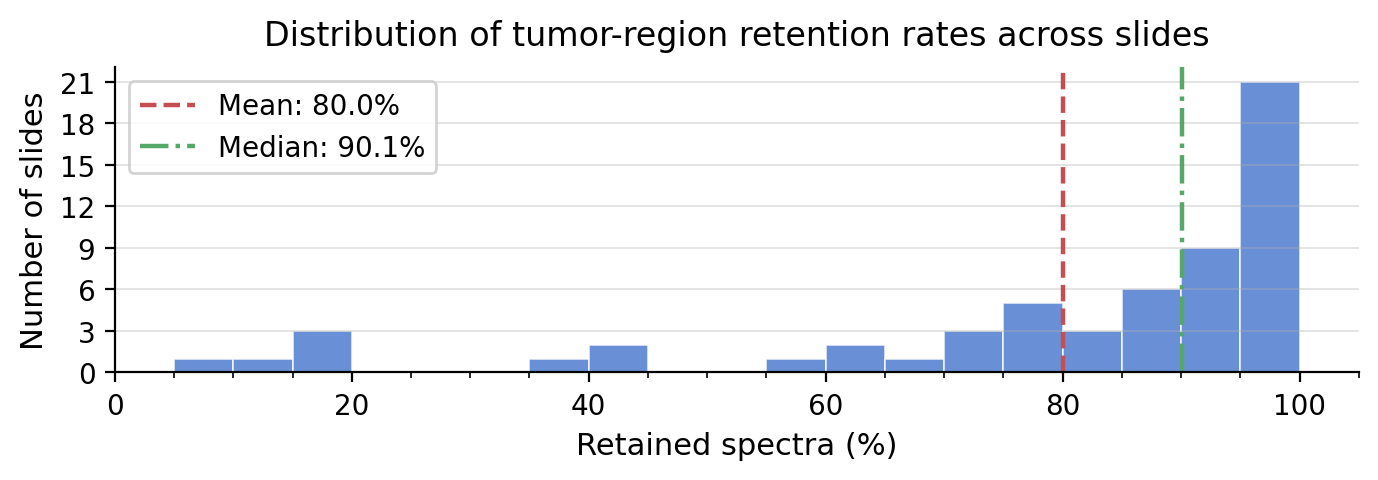
\includegraphics[width=\linewidth]{images/tumor_retention_histogram.png}
    \caption{Histogram of retention rates.}
    \label{fig:tumor_retention_rates}
\end{figure}

This approach ensured that each slide was processed independently and visually inspected to verify cluster consistency. The resulting binary tumor labeling yields approximately 200,000 spectra retained for downstream analysis from the original $\sim$270,000. We draw attention to the fact that the percentage of retained spectra from each slide varied significantly (see Fig. \ref{fig:tumor_retention_rates}). We note that the two step filtering of viable pixels, via a maximum intensity threshold followed by clustering has some degree of robustness; low signal quality spectra not filtered by the threshold will be filtered by the clustering and manual selection. On the other hand, as noted earlier, this pipeline is not standard or unique, but applies some common data processing techniques to the given problem under assuptions like spatial cohesiveness or spectral similarities.


\section{Deep Generative Augmentation}
\label{sec:cvae_architecture}
To learn the underlying distribution of tumor spectra, we implemented a 1D-Convolutional Conditional Variational Autoencoder ($\beta$-CVAE). 1D convolutions were chosen to exploit the strong local dependencies between adjacent Raman shift frequencies (e.g., the broad lipid/protein bands between $1400$ and $1500 \text{ cm}^{-1}$). 

As illustrated in Figure \ref{fig:cvae_architecture}, the architecture is composed of an encoder, a $d$-dimensional latent bottleneck, and a decoder. The encoder $q_\phi(z|x)$ compresses the input Raman spectrum $x$ into a latent representation $z$. To encourage class separation in the reconstructed spectra, $\hat{x}$, we conditioned the decoder $p_\theta(\hat{x}|z,y)$ on the class label $y$ provided as a one-hot encoded vector. 

To ensure that the encoder learns class discriminative features, we framed the encoding process as a Multi-Task Learning (MTL) problem by appending an auxiliary classification head to the encoder.
The model is optimized using a composite loss function:
\begin{equation}
\mathcal{L}_{\text{total}} = \mathcal{L}_{\text{recon}} + \beta \cdot D_{KL}(q_\phi(z|x) \| p(z)) + \alpha \cdot \mathcal{L}_{\text{class}}. 
\end{equation}

$\mathcal{L}_{\text{recon}}$ represents the reconstruction loss, and is defined as
\begin{align}
\mathcal{L}_{\text{recon}} &= \gamma \cdot \text{MSE}(x, \hat{x}) + (1 - \gamma) \cdot \text{CosineLoss}(x, \hat{x}) \\
\nonumber &= \gamma \cdot \frac{1}{N_{\lambda}} \| x - \hat{x} \|_2^2 + (1 - \gamma) \cdot \left(1 - \frac{x \cdot \hat{x}}{\|x\|_2 \|\hat{x}\|_2}\right). 
\end{align} 
We performed multiple experiment and we tested with values of $\gamma \in \{0, 0.5, 1\}$.

$\mathcal{L}_{\text{class}}$ represents the categorical cross-entropy loss of the auxiliary classifier: 
\begin{equation}
\mathcal{L}_{\text{class}} = - \sum_{c=1}^{C} y_c \log(p_c),
\end{equation} where $y_c$ is the true label and $p_c$ the predicted probability associated with class $c$. The categorical cross-entropy loss is scaled by $\alpha$; in our experiments, we set $\alpha \le 0.5$ empirically, as the classification task is auxiliary and included only for training the encoder. We observed that scaling by a factor $\alpha = 0.5$ led to overfitting the encoder on the classification task very early during training, therefore we chose $\alpha = 0.2$ which led to a similar rate of convergence across the classification and the reconstruction tasks.

The parameter $C \in \{2, 6\}$ denotes the number of label classes, $C=2$ for binary classification (IDH-mutant, IDH-wildtype), or $C = 6$ for classifying all six glioma sub-types.

Once trained, the decoder can generate class-balanced synthetic datasets
by sampling $z \sim \mathcal{N}(0, I)$ conditioning on a requested class label.

\begin{figure}[h]
    \centering
    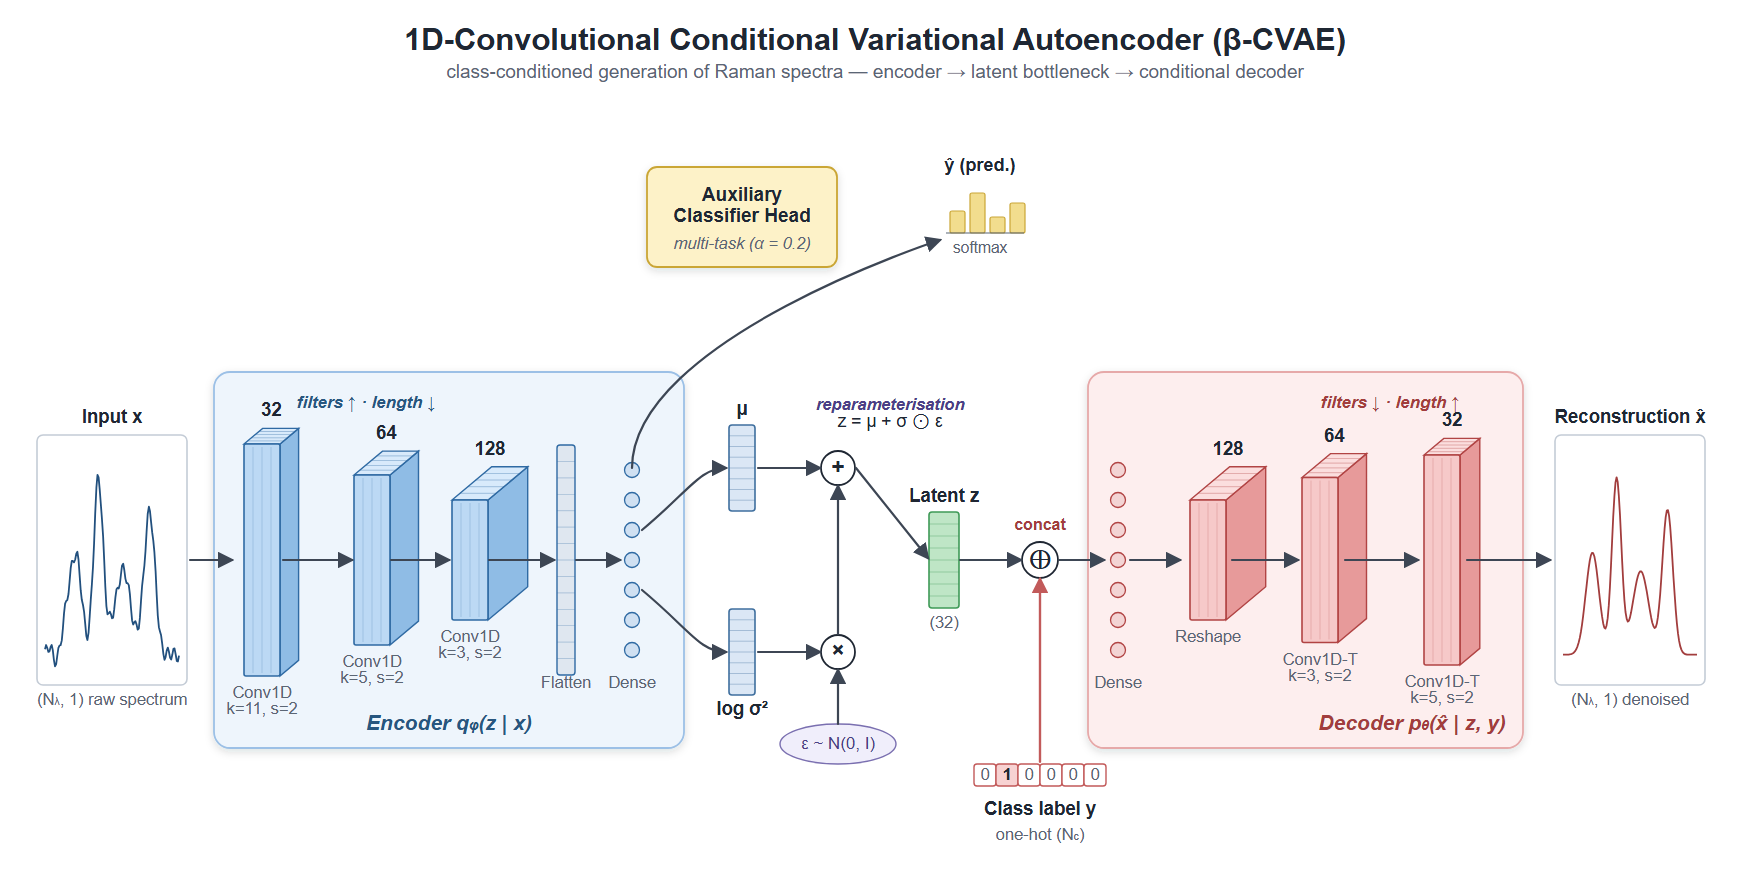
\includegraphics[width=\linewidth]{images/cvae_architecture.png}
    \caption{\footnotesize Architecture of the 1D-Convolutional Conditional Variational Autoencoder ($\beta$-CVAE). The encoder is composed of 1-d convolutional layers with 3 blocks: filters $[32, 64, 128]$, kernels $[11, 5, 3]$, and strides $[2, 2, 2]$, compressing the input spectrum to the $d$-dimensional latent space. The decoder reconstructs the spectrum conditioned on both the latent representation and the class label, using transpose convolutions with initial filters of 128, followed by 3 blocks with filters $[128, 64, 32]$, kernels $[3, 5, 11]$, and strides $[2, 2, 2]$. 
    %The model is trained with batch size 256 for 70 epochs at learning rate $0.001$ with reconstruction loss mode MSE, generating 20,000 samples per class.  
    An auxiliary classifier head is attached to the encoder to encourage the convolutional layers to capture class discriminative features.}
    \label{fig:cvae_architecture}
\end{figure}

Following the $\beta$-VAE framework introduced by Higgins et al. \cite{higgins2017betavae}, the Kullback-Leibler divergence ($D_{KL}$) acts as a structural regularizer when scaled by $\beta>1$. 

For a Gaussian distribution regularizer, the divergence has the following expression \cite{higgins2017betavae, Asperti2020}:
\begin{equation}
D_{KL}(q_\phi(z|x) \| p(z)) = \frac{1}{2} \sum_{i=1}^{d} \left( \mu_i^2 + \sigma_i^2 - \log(\sigma_i^2) - 1 \right).
\end{equation}

According to Higgins et al., a higher weight for the divergence term ensures that the latent space is sufficiently regularized, which constitutes a requirement for the generator to be used by sampling from a normal distribution \cite{higgins2017betavae}, hence we set $\beta=2$. The latent vector $z \in \mathbb{R}^d$ has two $d$-dimensional parameters associated: $\mu$ and $\log(\sigma^2)$. In our experiments, we tested $d \in \{ 16, 32, 64 \}$, but most of the experiments used $d=32$.


\section{Classification by Reconstruction}
\label{sec:cbr}


Standard discriminative models such as Random Forests and XGBoost optimize class-separating decision boundaries from labeled training data. However, in small-cohort Raman spectroscopy settings, these models may generalize poorly to unseen samples affected by acquisition variability and changing spectrometer baselines. Motivated by this limitation, we investigate an alternative generative inference strategy, termed Classification by Reconstruction (CbR).

CbR leverages the CVAE's learned latent representations to classify a tumor without relying on discriminative boundaries. 
During inference on a preprocessed unseen test spectrum $x_{\text{test}}$, we defined the following approach:
\begin{enumerate}
    \item \emph{Latent extraction.} The test spectrum is passed through the encoder to extract its latent vector: $\mu_{z} = \text{Encoder}(x_{\text{test}})$.
    \item \emph{Conditional reconstruction.} The latent vector $\mu_{z}$ is passed to the decoder $C$ times. Each forward pass pairs $\mu_{z}$ with a different one-hot class condition $y_c$, generating a set of reconstructed spectra: \\ $\hat{x}_c = \text{Decoder}(\mu_{z}, y_c)$.
    \item \emph{Error minimization.} We compute the MSE between the raw test spectrum and each of the reconstructions. The final predicted class $\hat{y}$ is the one that yields the lowest reconstruction error:
    \begin{equation}
    \hat{y} = \underset{c \in \{1, \dots, C\}}{\arg \min} \left( \| x_{\text{test}} - \hat{x}_c \|_2^2 \right).
    \end{equation}
\end{enumerate}

This approach assumes that spectra reconstructed under the correct class condition will exhibit lower reconstruction error than spectra reconstructed under incorrect class conditions.

\chapter{Experimental Design}
\label{sec:experimental_design}

All experiments were conducted using a strict patient-level 5-fold design (see Appendix \ref{app:cv_schema}), ensuring that no patient contributed tissue to both the training and the evaluation set of a fold, while keeping class balance into account. Since several patients supplied more than one tissue section, this is a stronger guarantee than separating individual slides. We evaluated the proposed framework under three complementary settings: Train-on-Real, Test-on-Real (TR/TR), Train-on-Synthetic, Test-on-Real (TS/TR), and Train-on-Synthetic+Real, Test-on-Real (TSR/TR) \cite{esteban2017real}. We also evaluated the proposed Classification by Reconstruction (CbR) strategy as a reconstruction-based generative inference approach.

\section{Classification Tasks}

To evaluate the impact of biological signal strength on classification performance, all models were evaluated on two distinct tasks:
\begin{enumerate}
    \item \emph{Binary classification (IDH-Status).} Differentiating the IDH-Mutant from the IDH-Wildtype entails a large metabolic shift that is theoretically easier to detect above spectrometer noise.
    \item \emph{6-class grading.} Differentiating all six distinct glioma sub-grades is a more challenging task, as the biochemical differences between sub-grades are more subtle and the signal may not capture them.
\end{enumerate}

\section{Evaluation Protocols}
\paragraph{TR/TR Evaluation.} 
We established the real-data baseline using the Train-on-Real, Test-on-Real (TR/TR) paradigm. The training splits consisted exclusively of real spectra from the training folds. We evaluated four downstream classifiers:
\begin{enumerate}
    \item \emph{RF + SVM:} A Random Forest feature selector (top 20 bands) followed by a Support Vector Machine with RBF kernel and balanced class weights \cite{apollonov2024raman}.
    
    \item \emph{Random Forest:} A standard ensemble of 100 trees with balanced class weights.
    
    \item \emph{XGBoost:} A gradient-boosted tree ensemble utilizing histogram-based tree methods optimized for high-dimensional data.
    
    \item \emph{1D-CNN:} A deep convolutional classifier trained with early stopping.
\end{enumerate}

\paragraph{TS/TR Evaluation.}
To evaluate whether the CVAE captured discriminative structure from the training data, we employed the Train-on-Synthetic, Test-on-Real (TS/TR) framework. For each fold, the CVAE was trained exclusively on the corresponding real training split. By sampling from the latent prior $z \sim \mathcal{N}(0, I)$, the decoder was then used to generate synthetic spectra conditioned by class (40,000 for binary tasks and 120,000 for 6-class tasks) in almost all experiments, except in the TSR/TR ratio ablation study (see Table \ref{tab:appendix_exp_401} in Appendix). The downstream classifiers were trained exclusively on synthetic spectra and evaluated on the corresponding held-out real validation fold.

\paragraph{TSR/TR Evaluation.}
We also evaluated a Train-on-Synthetic+Real, Test-on-Real (TSR/TR) framework in which synthetic spectra were combined with the real training data. This setting evaluates whether synthetic augmentation improves classification performance relative to the TR/TR baseline.

\paragraph{CbR Evaluation.}
Finally, the proposed Classification by Reconstruction (CbR) inference strategy was evaluated on the held-out real validation folds. Reconstruction-based predictions were compared directly against the TR/TR and TS/TR baselines.

\section{Training Details}
We present here the specific details of our training setup. We note that the ML models were not tuned, as the focus of this study is the effect of data augmentation, not tuning the best classifiers. Most of our experiments are ablation designs where we test the effect on the accuracy.
\begin{enumerate}
    \item \textit{Spectrum region crop.} In all our experiments, we cropped the spectra to the fingerprint region ($700 - 1800 \text{ cm}^{-1}$) \cite{Harris2023}, thus we selected 571 spectral bands out of the $N_\lambda = 1738$. 
    \item \textit{Maximum number of spectra cap per slide.} We randomly drew a sample of a maximum of 500 spectra from each slide, ensuring that the slides are equally represented. We performed this operation to mitigate the high variability in the number of spectra per slide due to varying slide sizes and varying retention rates due to quality (see Fig. \ref{fig:tumor_retention_rates}). We drew a fixed sample for the classifiers and opted for a dynamic resampling for the CVAE training.
    \item \textit{CVAE training data augmentation:} We performed dynamic data augmentation at train time using the following operations: 
    (a) \textit{within-class mixup:} we used linear combinations of spectra within the same class to expand the input space; $x = \lambda x_1 + (1-\lambda) x_2$, with $\lambda \sim U(0,\alpha)$, and we set $\alpha = 0.5$; 
    (b) \textit{spectral shift:} we shifted the spectra by a random integer in $[-\text{max\_shift},+\text{max\_shift}]$ to simulate Raman calibration drift; we set $\text{max\_shift}=3$ in our experiments.
\end{enumerate}


\section{Statistical Evaluation}
\label{sec:statistical_eval}

Two protocols in this work group spectra into clusters, and they deliberately use different
units. It is worth stating the distinction explicitly, since both are referred to as
``clustering'' of the data and they serve different purposes.

\emph{Data splitting is performed at the patient level.} No patient contributes tissue to both
the training and the evaluation side of any fold (Section~\ref{sec:cv_design}). The purpose here
is to guarantee that evaluation data is genuinely unseen, so the correct unit is the strictest
one available: a model must not be tested on a patient it has already been shown, regardless of
which tissue section that patient supplied. Every accuracy reported in this work is obtained
under this constraint.

\emph{Uncertainty estimation is performed at the slide level.} The bootstrap described below
resamples whole slides rather than whole patients. The purpose here is different: not to prevent
leakage, but to estimate how much a reported metric would vary if the study were repeated. Each
slide corresponds to one Raman acquisition on one tissue section, and the dominant sources of
variation between measurements, i.e., instrument state, focusing, calibration drift, and sample
preparation, act at the level of the acquisition rather than at the level of the patient. Since
the object under evaluation is a spectral generator, we regard the acquisition session as the
natural exchangeable cluster, and resampling slides simulates the variability that a fresh batch
of acquisitions would produce. This is a deliberate relaxation relative to the splitting
protocol: where a single patient contributed several sections, those sections are treated as
exchangeable during resampling, which we consider appropriate for characterising spectral
variability even though it would not be appropriate for constructing a test set.

Due to the hierarchical structure of the dataset, individual spectra originating from the same
biopsy sample are strongly correlated. Consequently, statistical evaluation at the
individual-spectrum level violates the independent and identically distributed (I.I.D.)
assumption and may artificially underestimate uncertainty. Conversely, estimating variance solely
across the five cross-validation folds yields limited statistical power.

To obtain more robust uncertainty estimates, we implemented a stratified cluster bootstrap
procedure at the slide level. Across 1,000 bootstrap iterations, slides were sampled with
replacement while preserving class proportions. This procedure preserves the correlation
structure within each slide while approximating variability across independent batches of biopsy
slides.

For pairwise comparisons between evaluation settings (TS/TR vs. TR/TR or TSR/TR vs. TR/TR), we computed bootstrap distributions of the corresponding accuracy differences:
\[
\Delta = \mathrm{Accuracy}_{A} - \mathrm{Accuracy}_{B}.
\]

Statistical significance was evaluated using bootstrap $p$-value estimates. Confidence Intervals (CI) were determined using the bootstrap distribution, and a result is considered significant when the 95\% CI around $\Delta$ excludes zero. The two sided $p$-value is defined as \[p = 2 \cdot \min\!\left(\frac{\# \{ i = \overline{1, N} : \Delta_i<0\}}{N},\frac{\#\{i = \overline{1, N} :\Delta_i>0\}}{N}\right),\] where $N = 1,000$. We note that no statistical correction is applied for multiple tests across the suite of experiments or classifiers; this is an important limitation and inflates the Type~I error rate.


\chapter{Results}
\label{sec:results}

We performed a series of experiments to determine the effects of different design choices on the domain gap metric. Specifically, we tested (a) the reconstruction loss function (MSE, CosineLoss, or a combination of them), (b) the latent space dimension, and (c) the real-to-synthetic data ratio. Detailed results can be found in Appendix A. The main findings are presented below.

\section{Binary IDH Classification}
\label{sec:results_binary}

The binary classification is influenced by broad metabolic differences that can be detected using RS. Under the TR/TR setting, the best-performing discriminative models achieved accuracies above $70\%$ (see Table \ref{tab:binary_results}).

\begin{table}[h] 
\caption{Binary classification results for experiment \texttt{exp\_201} (CVAE with MSE reconstruction loss, latent dimension $d=32$, $\beta=2$).}
\label{tab:binary_results}
\small
\begin{tabular*}{\textwidth}{@{\extracolsep{\fill}}llcccc}
\toprule
\emph{Model} & \emph{Regimen} & \emph{Bal. Acc.} & \emph{$\Delta$} & \emph{95\% CI} & \emph{Macro F1}\\
\midrule
\multirow{3}{*}{RF + SVM} & TR/TR & $0.688$ & -- & -- & $0.765$ \\
 & TS/TR & $0.431$ & $-0.257$* & $[-0.330, -0.180]$ & $0.926$ \\
 & TSR/TR & $0.699$ & $+0.011$ & $[-0.015, +0.037]$ & $0.775$ \\
\midrule
\multirow{3}{*}{RF} & TR/TR & $0.734$ & -- & -- & $0.782$ \\
 & TS/TR & $0.669$ & $-0.065$ & $[-0.148, +0.017]$ & $0.764$ \\
 & TSR/TR & $0.742$ & $+0.008$ & $[-0.001, +0.019]$ & $0.785$ \\
\midrule
\multirow{3}{*}{XGBoost} & TR/TR & $0.742$ & -- & -- & $0.788$ \\
 & TS/TR & $0.622$ & $-0.120$* & $[-0.191, -0.051]$ & $0.737$ \\
 & TSR/TR & $0.746$ & $+0.004$ & $[-0.004, +0.013]$ & $0.792$ \\
\midrule
\multirow{3}{*}{1D-CNN} & TR/TR & $0.588$ & -- & -- & $0.875$ \\
 & TS/TR & $0.398$ & $-0.190$* & $[-0.299, -0.077]$ & $0.774$ \\
 & TSR/TR & $0.602$ & $+0.014$ & $[-0.055, +0.086]$ & $0.730$ \\
\midrule
CbR & -- & $0.619$ & -- & $[+0.548, +0.681]$ & $0.727$ \\
\bottomrule
\end{tabular*}
\small{Regimens: TR/TR (real-only baseline), TS/TR (synthetic-only), TSR/TR (synthetic + real), CbR (Classification by Reconstruction, model-independent). All figures are slide-level (per-(class, slide) stratified mean, matching the bootstrap): Bal. Acc. is slide-level balanced accuracy and Macro F1 is the slide-level macro-averaged F1. $\Delta$ and 95\% CI are the slide-level bootstrap difference vs.\ TR/TR; (*) marks a 95\% CI excluding zero. The CbR row reports its own accuracy 95\% CI.}
\end{table}

Across all classifiers, models trained exclusively on synthetic spectra underperformed the corresponding TR/TR baselines, which implies a substantial domain gap between synthetic and real spectra. Nevertheless, the performance degradation remained relatively moderate for RF and XGBoost, suggesting that the generated spectra retain part of the discriminative structure of the original data distribution.

In contrast to the TS/TR setting, combining synthetic and real spectra generally improved downstream classification performance. The largest improvement was observed for the 1D-CNN model; Random Forest and XGBoost also showed positive trends. This indicates that synthetic spectra are more effective as a regularization mechanism, augmenting real training data, than as a complete replacement for real measurements.

Of particular interest is the CbR inference method, which reached an accuracy of around 62\%. While lower than the other classifiers' accuracies, it is in the same range as the TS/TR models.

\section{6-Class Glioma Sub-Grading}
\label{sec:results_6class}


The 6-class glioma sub-grading task proved more challenging than binary IDH-status classification. Under the TR/TR setting, the best-performing models achieved accuracies of approximately $30\%$. Such results pinpoint the difficulty of detecting spectral differences at glioma sub-grades granularity. The outcomes of the 6-class experiments can be found in Appendix A (see Tables \ref{tab:appendix_exp_204}--\ref{tab:appendix_exp_206}).

Across all classifiers, training exclusively on synthetic spectra resulted in lower performance than the corresponding TR/TR baselines, reiterating the gap between generated and real spectra. The reduction in performance was more pronounced than in the binary setting, suggesting that subtle inter-class biological differences are more difficult to reproduce through synthetic generation in this small cohort setting.

\section{Remarks}
Despite the limitations observed in the TS/TR setting, augmenting the real training data with synthetic spectra generally improved downstream classification performance slightly. In nearly all experiments, RF and XGBoost were the most robust, with the lowest domain gaps and most consistent outcomes across experiments, with results over 70\% for TR/TR, over 60\% for TS/TR and slight improvements over the baseline for TSR/TR.

The accuracies of 1D-CNN were less consistent, showing a tendency of improvement with larger training datasets (see Tables \ref{tab:appendix_exp_401}--\ref{tab:appendix_exp_403}).

We note that, given our large number of model comparisons, for a rigorous statistical evaluation, a correction on the statistical significance should be applied. However, given that most of our results reveal mostly small and not statistically significant improvements, we decided not to perform any correction and discuss the results only as general tendencies.

\chapter{Discussion}
 \label{sec:discussion}

The experiments show that synthetic augmentation can slightly improve Raman-based glioma classification. However, they also reveal a substantial domain gap between generated and real spectra, especially in the 6-class grading task.

Combining synthetic and real spectra in the TSR/TR setting generally improved downstream classification performance across multiple models. This showcases the potential of synthetic spectra to improve the generalization capabilities of downstream models used in small-cohort settings. Therefore, instead of relying on synthetic spectra as a complete replacement for real measurements, they might be of greater use as a regularization strategy. 

To characterize the relationship between the real and synthetic spectral distributions beyond aggregate classification metrics, we examined two complementary embedding methods: PCA and $t$-SNE. Both were computed on $z$-scored, pooled real and synthetic spectra (up to $2000$ spectra per class per source). $t$-SNE was applied to the top $50$ principal components due to the high dimensionality ($N_\lambda$) of the input space. Each embedding is displayed twice: coloured by source (real vs.\ synthetic) and by diagnostic class (IDH-Mutant vs.\ IDH-Wildtype). The results are shown in Figure~\ref{fig:pca_tsne}.

\begin{figure}[h]
    \centering
    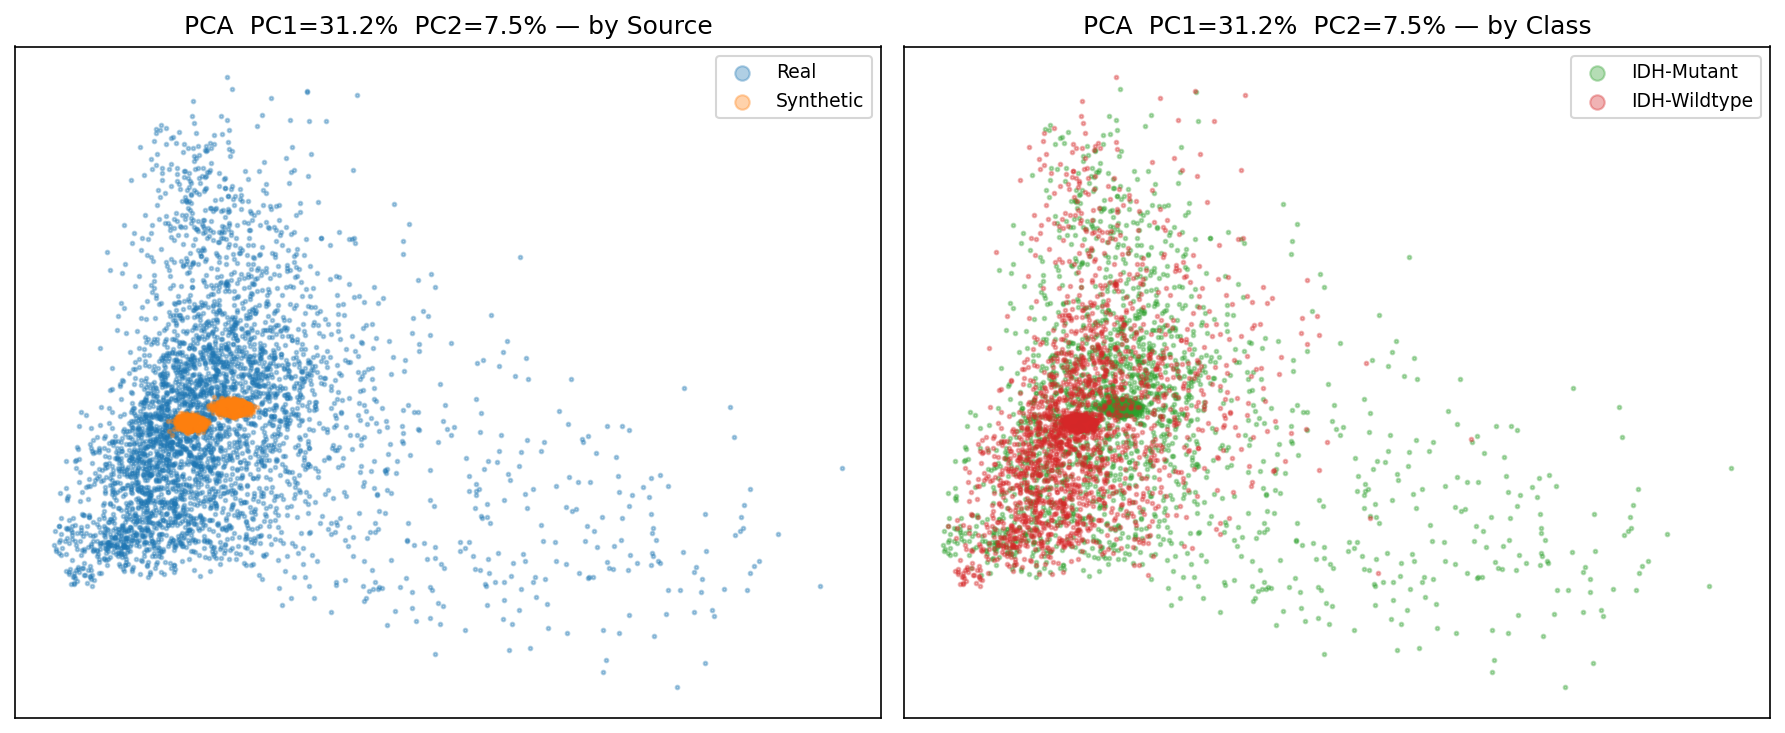
\includegraphics[width=\textwidth]{images/PCA.png}\\[4pt]
    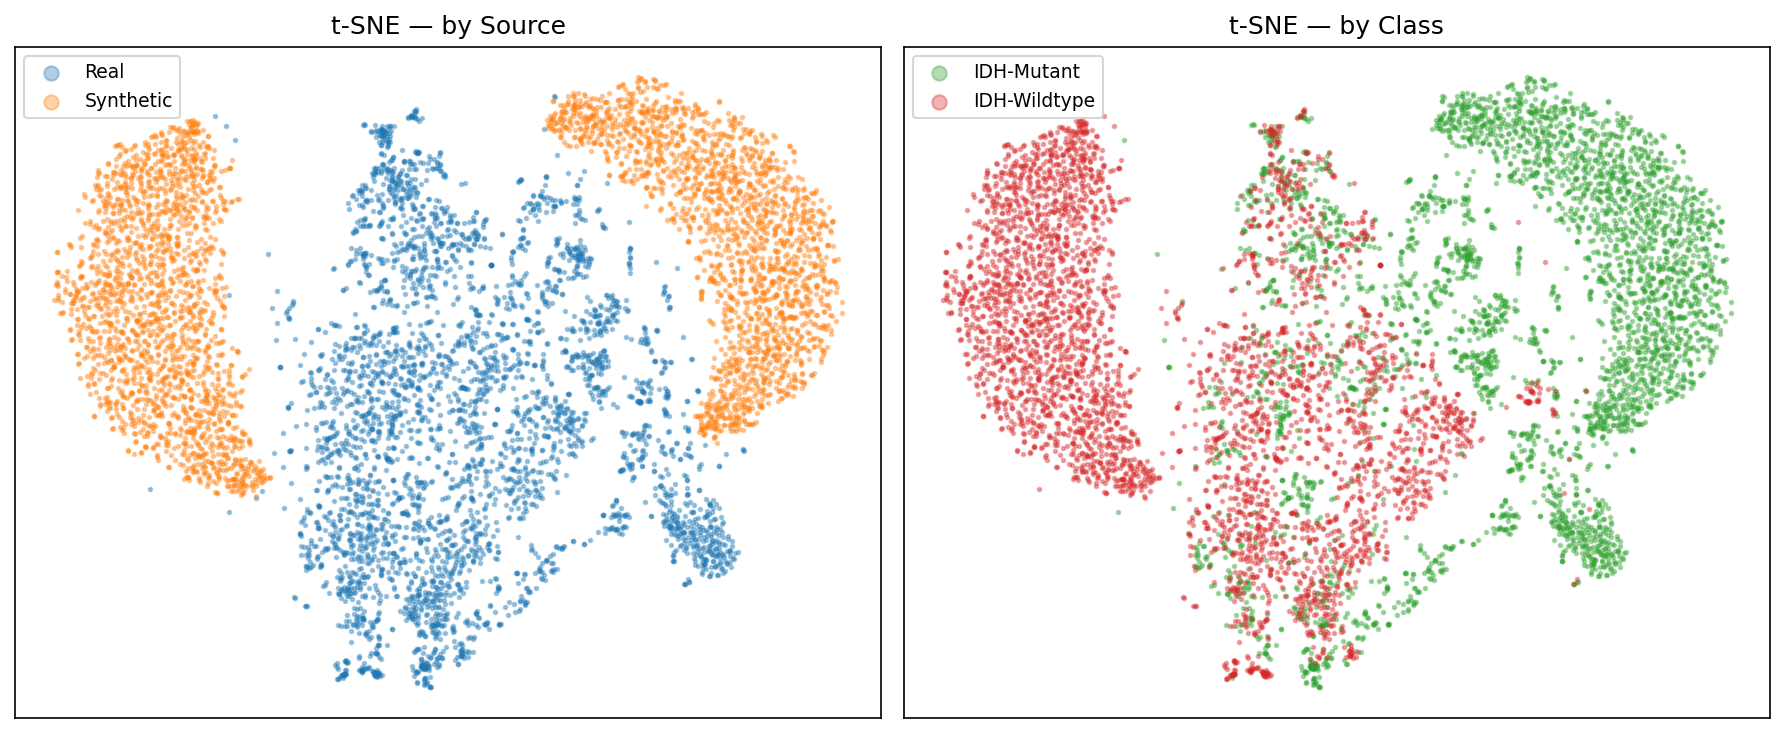
\includegraphics[width=\textwidth]{images/TSNE.png}
    \caption{\footnotesize PCA (top) and $t-$SNE (bottom) embeddings of real and synthetic spectra, coloured by source (left) and class (right).}
    \label{fig:pca_tsne}
\end{figure}

Taken together, the PCA and t-SNE plots offer insight into the spatial structure of the spectral data. The PCA plots reveal a variance difference between the real and the synthetic data sets: synthetic data forms two distinct clusters (corresponding to the two classes) with low variance, while the real data shows higher variance, and the two classes overlap to a great extent. Correlating these plots with the t-SNE plots, we can see that synthetic data is structured in two distinct clusters, whereas the raw data has a heterogeneous structure. It is worth noting that both the PCA and the t-SNE plots show the real data being intertwined. We hypothesize that the two classes might overlap (in the initial space) to such an extent that, under a strict, slide-isolated experiment, the possible accuracy for this particular dataset has a definite upper bound. 

We can visualize the spectral variance by plotting the mean spectrum of the real data and that of the synthetic data along with their standard deviation ($\sigma$) envelopes. We observe that the synthetic data standard deviation is much narrower than that of the real data, which suggests that the synthetic data is generally very close to the mean spectrum (Fig. \ref{fig:mean_std_spectra}).

\begin{figure}[h]
\centering
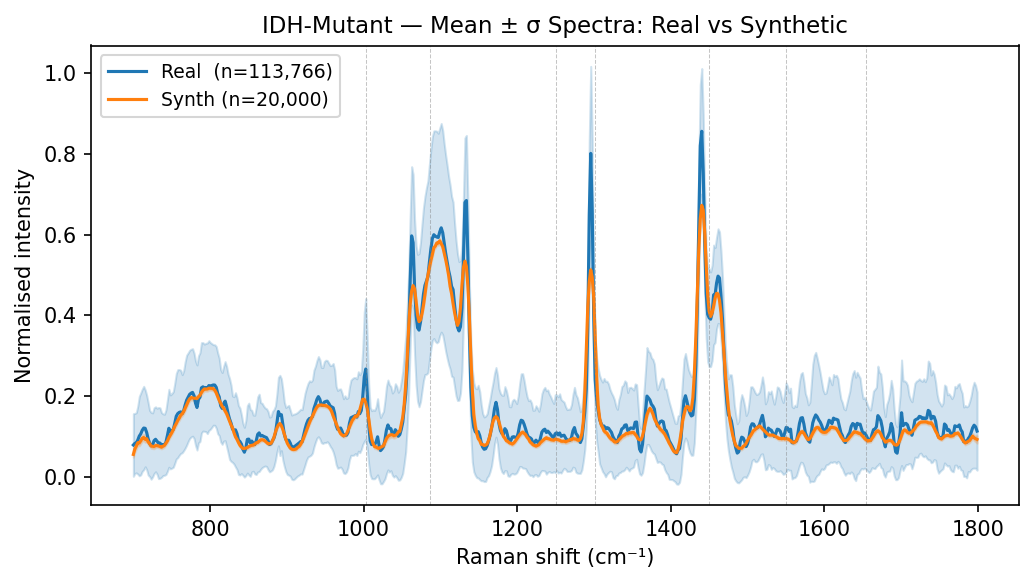
\includegraphics[width=0.85\textwidth]{images/A_mean_std_spectra_IDH-Mutant.png}
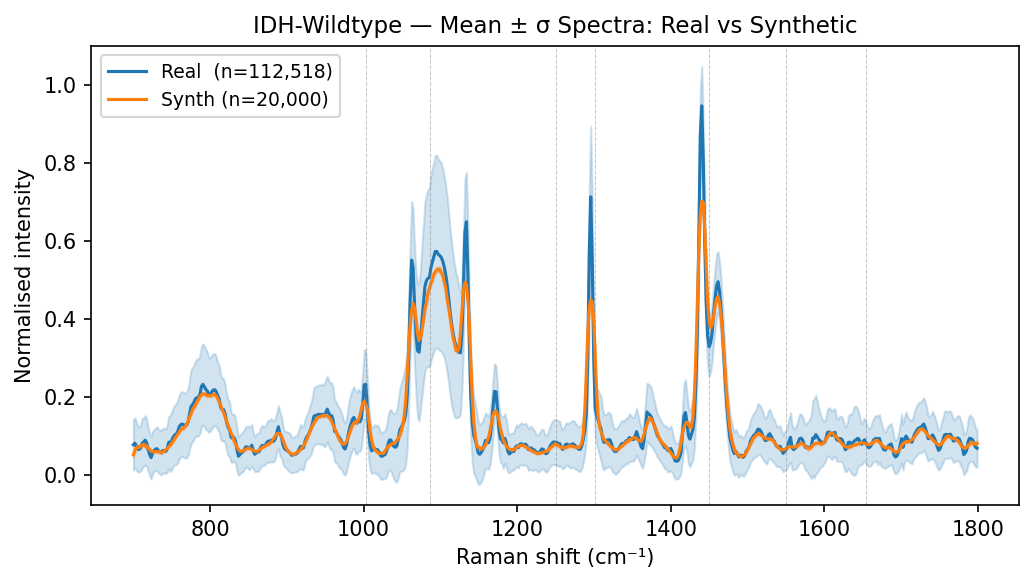
\includegraphics[width=0.85\textwidth]{images/A_mean_std_spectra_IDH-Wildtype.png}
\caption{Mean $\pm \sigma$ Raman spectra, real vs. synthetic, per class.}
\label{fig:mean_std_spectra}
\end{figure}

An important observation is that useful augmentation effects were obtained despite the relatively small number of independent patient samples available for training the generative model. In contrast to conventional deep generative modeling settings involving very large datasets, biomedical Raman spectroscopy typically operates in a data-constrained regime characterized by limited patient cohorts, acquisition variability, and strong intra-sample correlations. The present results indicate that generative models may still capture sufficient spectral structure to improve downstream robustness even when trained under these constraints.

The proposed Classification by Reconstruction (CbR) framework further demonstrates that the learned latent representations retain class-relevant spectral information. Although reconstruction-based inference did not outperform discriminative classifiers, its performance remained comparable to the TS/TR setting, suggesting that the generative model captures part of the discriminative structure of the underlying data distribution. More broadly, these results indicate that reconstruction-based inference may provide an alternative perspective for evaluating generative representations in biomedical spectroscopy.

\section{Limitations and Future Work}
\label{sec:limitations}

Several limitations remain. The dataset size is modest in terms of independent slide samples, and all experiments were conducted on a single acquisition setting. Moreover, the proposed spatio-spectral annotation pipeline includes heuristic and visually guided components that may introduce selection bias. The observed domain gap between synthetic and real spectra further indicates that the current CVAE architecture does not fully capture the variability present in the real data distribution, particularly for subtle multi-class grading tasks.

Future work could investigate larger multi-site datasets, alternative generative architectures such as diffusion-based models, and more systematic evaluation of synthetic spectrum fidelity and diversity. Additional directions include improving reconstruction-based inference strategies and exploring latent-space regularization methods better suited for highly heterogeneous biomedical spectral data.

\chapter{Conclusion}
\label{ch:conclusion}

The present study supports the use of synthetic augmentation to improve model robustness in small-cohort Raman spectroscopy studies and highlights the potential of generative modeling as a complementary strategy for addressing data scarcity in biomedical spectral diagnostics. 

In this work, we addressed the problem of data scarcity in Raman spectroscopy-based glioma classification by developing a conditional variational autoencoder capable of generating class-conditioned synthetic spectra. We have designed and applied a spatio-spectral preprocessing pipeline to extract tumor-spectra from $58$ glioma biopsy slides, combining median filtering, NMF-based clustering, and GMM-guided visual selection. The conditional VAE was trained under a multi-task objective that jointly optimized spectral reconstruction and auxiliary class discrimination, with a KL-regularized latent space to support generative sampling. Synthetic spectra were evaluated under TS/TR and TSR/TR protocols within a strict slide-isolated cross-validation scheme across four downstream classifiers, i.e., RF+SVM, Random Forest, XGBoost, and $1$D-CNN, on both binary IDH-status and $6$-class methylation subtype tasks. We have also proposed and evaluated Classification by Reconstruction (CbR) as a generative inference strategy that bypasses discriminative classifiers entirely. We gained the insight that, whereas synthetic spectra were not able to substitute for real data, they are useful as an augmentation data tool in order to improve classification robustness.

\section*{Summary of contributions}

\TODO{Mirror the contributions list in Chapter~\ref{ch:background}'s preceding introduction,
but written in the past tense and with the outcome of each attached rather than the promise.
Keep the two lists in correspondence: a reader should be able to check each claim made at the
start against what was actually delivered.}

\section*{What the evidence does and does not support}

\TODO{This section is what distinguishes a defensible conclusion from a summary, and it is
worth being precise. The honest reading of Chapter~\ref{sec:results}:

\emph{Supported.} Synthetic augmentation in the TSR/TR regime shifts accuracy upward
consistently in sign across models and both tasks. The generator captures class-mean spectral
structure well enough for a classifier trained on synthetic data alone to stay well above
chance (RF reaches $0.669$ against a $0.734$ real baseline in
Table~\ref{tab:binary_results}). CbR performs comparably to TS/TR, indicating the latent
space retains class-relevant information.

\emph{Not supported.} That the TSR/TR improvements are statistically distinguishable from
zero: of the four binary models, none has a 95\% CI excluding zero
(Table~\ref{tab:binary_results}), and the same holds in the six-class task
(Table~\ref{tab:sixclass_results}). The consistent \emph{sign} across models and tasks is
suggestive, and the honest formulation is that these are tendencies rather than demonstrated
effects. Note also that no correction for multiple comparisons is applied
(Section~\ref{sec:statistical_eval}), which if anything makes the individual intervals
optimistic.

\emph{Refuted, or at least clearly not achieved.} That synthetic spectra can substitute for
real ones: TS/TR is below TR/TR for every model in both tasks, significantly so in most.

Resist the temptation to soften the middle category -- a thesis that states plainly which of
its own results are inconclusive is stronger at a defence, not weaker.}

\section*{Outlook}

\TODO{Two or three sentences pointing forward, and cross-reference
Section~\ref{sec:limitations} rather than repeating it. The most concrete next step suggested
by this work's own evidence is a $\beta$ sweep: Chapter~\ref{sec:discussion} identifies
variance collapse as the specific failure, and $\beta$ is the parameter that trades latent
regularisation against reconstruction diversity. It was held at $2.0$ in every experiment.}



\printbibliography[heading=bibintoc]

\newpage
\appendix
\addcontentsline{toc}{chapter}{\textbf{Appendices}} 
\begin{appendices}

    % =====================================================================
% FROZEN - do not regenerate this file.
%
% paper/gen_appendix_tables.py writes to "paper/appendix (5).tex", not
% here. Running it against this file would lose:
%   - the hand-corrected exp_302 / exp_303 captions (latent-dimension
%     ablation; the generator copies the registry description, which
%     mislabelled them as a reconstruction-loss ablation until 2026-09-03)
%   - Appendix B, the Stratified Evaluation Protocol, which is written
%     by hand and has no generator counterpart
%
% The experiment tables are final. Edit them here directly.
% =====================================================================

\appendix

\chapter{Extended Experiment Results}
\setcounter{table}{0}
\renewcommand{\thetable}{\Alph{chapter}.\arabic{table}}

This appendix reports the per-experiment, per-model results in full. Each table lists the slide-level balanced accuracy under each training regimen, the bootstrap difference $\Delta$ relative to the TR/TR baseline with its 95\% confidence interval, and the slide-level Macro F1, Sensitivity, Specificity. Unavailable entries are marked with a dash.

\section*{Experiments 201-206. Reconstruction Loss Ablation}
Experiments \texttt{201-206} are designed as an ablation test on the CVAE reconstruction loss function, measuring the effect of the tradeoff between MSE and CosineLoss reconstruction metrics. Experiments 201-203 correspond to binary tasks, and experiments 204-206 correspond to 6-class tasks.

\begin{table}[htp]
\centering
\scriptsize
\caption{Extended results for \texttt{exp\_201}: Reconstruction Loss Ablation: MSE-only (gamma=1, delta=0) for binary classification.}
\label{tab:appendix_exp_201}
\begin{tabular*}{\textwidth}{@{\extracolsep{\fill}}llcccccc}
\toprule
\emph{Model} & \emph{Regimen} & \emph{Acc.} & \emph{$\Delta$} & \emph{95\% CI} & \emph{Macro F1} & \emph{Sensit.} & \emph{Specif.}\\
\midrule
\multirow{3}{*}{RF + SVM} & TR/TR & $0.688$ & -- & -- & $0.765$ & $0.749$ & $0.608$\\
 & TS/TR & $0.431$ & $-0.257$* & $[-0.330, -0.180]$ & $0.926$ & $0.000$ & $1.000$\\
 & TSR/TR & $0.699$ & $+0.011$ & $[-0.015, +0.037]$ & $0.775$ & $0.769$ & $0.605$\\
\midrule
\multirow{3}{*}{RF} & TR/TR & $0.734$ & -- & -- & $0.782$ & $0.857$ & $0.572$\\
 & TS/TR & $0.669$ & $-0.065$ & $[-0.148, +0.017]$ & $0.764$ & $0.707$ & $0.620$\\
 & TSR/TR & $0.742$ & $+0.008$ & $[-0.001, +0.019]$ & $0.785$ & $0.858$ & $0.588$\\
\midrule
\multirow{3}{*}{XGBoost} & TR/TR & $0.742$ & -- & -- & $0.788$ & $0.854$ & $0.595$\\
 & TS/TR & $0.622$ & $-0.120$* & $[-0.191, -0.051]$ & $0.737$ & $0.583$ & $0.674$\\
 & TSR/TR & $0.746$ & $+0.004$ & $[-0.004, +0.013]$ & $0.792$ & $0.852$ & $0.607$\\
\midrule
\multirow{3}{*}{1D-CNN} & TR/TR & $0.588$ & -- & -- & $0.875$ & $0.919$ & $0.152$\\
 & TS/TR & $0.398$ & $-0.190$* & $[-0.299, -0.077]$ & $0.774$ & $0.186$ & $0.679$\\
 & TSR/TR & $0.602$ & $+0.014$ & $[-0.055, +0.086]$ & $0.730$ & $0.797$ & $0.346$\\
\midrule
CbR & -- & $0.619$ & -- & $[+0.548, +0.681]$ & $0.727$ & $0.659$ & $0.567$\\
\bottomrule
\end{tabular*}
\small{Regimens: TR/TR (real-only baseline), TS/TR (synthetic-only), TSR/TR (synthetic + real), CbR (Classification by Reconstruction, model-independent). $\Delta$ and 95\% CI are the slide-level bootstrap difference vs.\ TR/TR; (*) marks a 95\% CI excluding zero. Macro F1, Sensitivity, Specificity are slide-level (per-(class, slide) stratified mean, matching the bootstrap). The CbR row reports its own accuracy 95\% CI.}
\end{table}

\begin{table}[htp]
\centering
\scriptsize
\caption{Extended results for \texttt{exp\_202}: Reconstruction Loss Ablation: Balanced MSE+Cosine (gamma=0.5, delta=0.5) for binary classification.}
\label{tab:appendix_exp_202}
\begin{tabular*}{\textwidth}{@{\extracolsep{\fill}}llcccccc}
\toprule
\emph{Model} & \emph{Regimen} & \emph{Acc.} & \emph{$\Delta$} & \emph{95\% CI} & \emph{Macro F1} & \emph{Sensit.} & \emph{Specif.}\\
\midrule
\multirow{3}{*}{RF + SVM} & TR/TR & $0.688$ & -- & -- & $0.765$ & $0.749$ & $0.608$\\
 & TS/TR & $0.431$ & $-0.257$* & $[-0.330, -0.180]$ & $0.962$ & $0.000$ & $1.000$\\
 & TSR/TR & $0.698$ & $+0.010$ & $[-0.018, +0.041]$ & $0.768$ & $0.784$ & $0.585$\\
\midrule
\multirow{3}{*}{RF} & TR/TR & $0.734$ & -- & -- & $0.782$ & $0.857$ & $0.572$\\
 & TS/TR & $0.624$ & $-0.110$* & $[-0.197, -0.029]$ & $0.722$ & $0.757$ & $0.448$\\
 & TSR/TR & $0.738$ & $+0.004$ & $[-0.003, +0.012]$ & $0.783$ & $0.854$ & $0.585$\\
\midrule
\multirow{3}{*}{XGBoost} & TR/TR & $0.742$ & -- & -- & $0.788$ & $0.854$ & $0.595$\\
 & TS/TR & $0.626$ & $-0.116$* & $[-0.200, -0.039]$ & $0.724$ & $0.737$ & $0.480$\\
 & TSR/TR & $0.741$ & $-0.002$ & $[-0.007, +0.003]$ & $0.787$ & $0.850$ & $0.596$\\
\midrule
\multirow{3}{*}{1D-CNN} & TR/TR & $0.588$ & -- & -- & $0.875$ & $0.919$ & $0.152$\\
 & TS/TR & $0.404$ & $-0.185$* & $[-0.281, -0.081]$ & $0.806$ & $0.161$ & $0.724$\\
 & TSR/TR & $0.639$ & $+0.051$ & $[-0.034, +0.136]$ & $0.724$ & $0.578$ & $0.720$\\
\midrule
CbR & -- & $0.617$ & -- & $[+0.547, +0.677]$ & $0.727$ & $0.634$ & $0.594$\\
\bottomrule
\end{tabular*}
\small{Regimens: TR/TR (real-only baseline), TS/TR (synthetic-only), TSR/TR (synthetic + real), CbR (Classification by Reconstruction, model-independent). $\Delta$ and 95\% CI are the slide-level bootstrap difference vs.\ TR/TR; (*) marks a 95\% CI excluding zero. Macro F1, Sensitivity, Specificity are slide-level (per-(class, slide) stratified mean, matching the bootstrap). The CbR row reports its own accuracy 95\% CI.}
\end{table}

\begin{table}[htp]
\centering
\scriptsize
\caption{Extended results for \texttt{exp\_203}: Reconstruction Loss Ablation: Cosine-only (gamma=0, delta=1) for binary classification.}
\label{tab:appendix_exp_203}
\begin{tabular*}{\textwidth}{@{\extracolsep{\fill}}llcccccc}
\toprule
\emph{Model} & \emph{Regimen} & \emph{Acc.} & \emph{$\Delta$} & \emph{95\% CI} & \emph{Macro F1} & \emph{Sensit.} & \emph{Specif.}\\
\midrule
\multirow{3}{*}{RF + SVM} & TR/TR & $0.688$ & -- & -- & $0.765$ & $0.749$ & $0.608$\\
 & TS/TR & $0.431$ & $-0.257$* & $[-0.330, -0.180]$ & $1.000$ & $0.000$ & $1.000$\\
 & TSR/TR & $0.681$ & $-0.007$ & $[-0.039, +0.027]$ & $0.753$ & $0.782$ & $0.547$\\
\midrule
\multirow{3}{*}{RF} & TR/TR & $0.734$ & -- & -- & $0.782$ & $0.857$ & $0.572$\\
 & TS/TR & $0.651$ & $-0.084$ & $[-0.167, +0.000]$ & $0.717$ & $0.858$ & $0.376$\\
 & TSR/TR & $0.738$ & $+0.004$ & $[-0.003, +0.012]$ & $0.785$ & $0.849$ & $0.590$\\
\midrule
\multirow{3}{*}{XGBoost} & TR/TR & $0.742$ & -- & -- & $0.788$ & $0.854$ & $0.595$\\
 & TS/TR & $0.643$ & $-0.100$* & $[-0.163, -0.031]$ & $0.705$ & $0.901$ & $0.302$\\
 & TSR/TR & $0.742$ & $-0.000$ & $[-0.005, +0.005]$ & $0.790$ & $0.852$ & $0.598$\\
\midrule
\multirow{3}{*}{1D-CNN} & TR/TR & $0.588$ & -- & -- & $0.875$ & $0.919$ & $0.152$\\
 & TS/TR & $0.447$ & $-0.141$* & $[-0.213, -0.073]$ & $0.813$ & $0.059$ & $0.961$\\
 & TSR/TR & $0.722$ & $+0.134$* & $[+0.053, +0.215]$ & $0.792$ & $0.735$ & $0.706$\\
\midrule
CbR & -- & $0.662$ & -- & $[+0.594, +0.725]$ & $0.749$ & $0.802$ & $0.476$\\
\bottomrule
\end{tabular*}
\small{Regimens: TR/TR (real-only baseline), TS/TR (synthetic-only), TSR/TR (synthetic + real), CbR (Classification by Reconstruction, model-independent). $\Delta$ and 95\% CI are the slide-level bootstrap difference vs.\ TR/TR; (*) marks a 95\% CI excluding zero. Macro F1, Sensitivity, Specificity are slide-level (per-(class, slide) stratified mean, matching the bootstrap). The CbR row reports its own accuracy 95\% CI.}
\end{table}

\begin{table}[htp]
\centering
\scriptsize
\caption{Extended results for \texttt{exp\_204}: Reconstruction Loss Ablation: MSE-only (gamma=1, delta=0) for 6-class classification.}
\label{tab:appendix_exp_204}
\begin{tabular*}{\textwidth}{@{\extracolsep{\fill}}llcccccc}
\toprule
\emph{Model} & \emph{Regimen} & \emph{Acc.} & \emph{$\Delta$} & \emph{95\% CI} & \emph{Macro F1} & \emph{Sensit.} & \emph{Specif.}\\
\midrule
\multirow{3}{*}{RF + SVM} & TR/TR & $0.289$ & -- & -- & $0.400$ & $0.221$ & $0.851$\\
 & TS/TR & $0.102$ & $-0.186$* & $[-0.275, -0.094]$ & $0.333$ & $0.141$ & $0.829$\\
 & TSR/TR & $0.301$ & $+0.012$ & $[-0.012, +0.040]$ & $0.407$ & $0.195$ & $0.846$\\
\midrule
\multirow{3}{*}{RF} & TR/TR & $0.260$ & -- & -- & $0.341$ & $0.224$ & $0.849$\\
 & TS/TR & $0.200$ & $-0.060$* & $[-0.117, -0.000]$ & $0.293$ & $0.274$ & $0.853$\\
 & TSR/TR & $0.264$ & $+0.003$ & $[-0.005, +0.012]$ & $0.350$ & $0.222$ & $0.849$\\
\midrule
\multirow{3}{*}{XGBoost} & TR/TR & $0.268$ & -- & -- & $0.377$ & $0.198$ & $0.842$\\
 & TS/TR & $0.251$ & $-0.018$ & $[-0.072, +0.041]$ & $0.369$ & $0.289$ & $0.864$\\
 & TSR/TR & $0.266$ & $-0.002$ & $[-0.009, +0.004]$ & $0.363$ & $0.198$ & $0.842$\\
\midrule
\multirow{3}{*}{1D-CNN} & TR/TR & $0.224$ & -- & -- & $0.867$ & $0.151$ & $0.829$\\
 & TS/TR & $0.075$ & $-0.149$* & $[-0.240, -0.062]$ & $0.226$ & $0.133$ & $0.829$\\
 & TSR/TR & $0.249$ & $+0.025$ & $[-0.100, +0.158]$ & $0.399$ & $0.252$ & $0.851$\\
\midrule
CbR & -- & $0.271$ & -- & $[+0.227, +0.318]$ & $0.381$ & $0.271$ & $0.852$\\
\bottomrule
\end{tabular*}
\small{Regimens: TR/TR (real-only baseline), TS/TR (synthetic-only), TSR/TR (synthetic + real), CbR (Classification by Reconstruction, model-independent). $\Delta$ and 95\% CI are the slide-level bootstrap difference vs.\ TR/TR; (*) marks a 95\% CI excluding zero. Macro F1, Sensitivity, Specificity are slide-level (per-(class, slide) stratified mean, matching the bootstrap). The CbR row reports its own accuracy 95\% CI.}
\end{table}

\begin{table}[htp]
\centering
\scriptsize
\caption{Extended results for \texttt{exp\_205}: Reconstruction Loss Ablation: Balanced MSE+Cosine (gamma=0.5, delta=0.5) for 6-class classification.}
\label{tab:appendix_exp_205}
\begin{tabular*}{\textwidth}{@{\extracolsep{\fill}}llcccccc}
\toprule
\emph{Model} & \emph{Regimen} & \emph{Acc.} & \emph{$\Delta$} & \emph{95\% CI} & \emph{Macro F1} & \emph{Sensit.} & \emph{Specif.}\\
\midrule
\multirow{3}{*}{RF + SVM} & TR/TR & $0.289$ & -- & -- & $0.400$ & $0.221$ & $0.851$\\
 & TS/TR & $0.155$ & $-0.134$* & $[-0.217, -0.047]$ & $0.261$ & $0.230$ & $0.844$\\
 & TSR/TR & $0.306$ & $+0.017$ & $[-0.002, +0.037]$ & $0.420$ & $0.236$ & $0.850$\\
\midrule
\multirow{3}{*}{RF} & TR/TR & $0.253$ & -- & -- & $0.344$ & $0.227$ & $0.851$\\
 & TS/TR & $0.234$ & $-0.018$ & $[-0.074, +0.039]$ & $0.320$ & $0.279$ & $0.852$\\
 & TSR/TR & $0.261$ & $+0.009$ & $[-0.002, +0.020]$ & $0.353$ & $0.211$ & $0.846$\\
\midrule
\multirow{3}{*}{XGBoost} & TR/TR & $0.268$ & -- & -- & $0.377$ & $0.198$ & $0.842$\\
 & TS/TR & $0.253$ & $-0.015$ & $[-0.073, +0.040]$ & $0.370$ & $0.281$ & $0.856$\\
 & TSR/TR & $0.270$ & $+0.002$ & $[-0.004, +0.007]$ & $0.365$ & $0.183$ & $0.838$\\
\midrule
\multirow{3}{*}{1D-CNN} & TR/TR & $0.224$ & -- & -- & $0.597$ & $0.174$ & $0.831$\\
 & TS/TR & $0.160$ & $-0.064$ & $[-0.176, +0.048]$ & $0.391$ & $0.248$ & $0.843$\\
 & TSR/TR & $0.347$ & $+0.123$* & $[+0.005, +0.239]$ & $0.509$ & $0.354$ & $0.872$\\
\midrule
CbR & -- & $0.265$ & -- & $[+0.223, +0.309]$ & $0.377$ & $0.289$ & $0.854$\\
\bottomrule
\end{tabular*}
\small{Regimens: TR/TR (real-only baseline), TS/TR (synthetic-only), TSR/TR (synthetic + real), CbR (Classification by Reconstruction, model-independent). $\Delta$ and 95\% CI are the slide-level bootstrap difference vs.\ TR/TR; (*) marks a 95\% CI excluding zero. Macro F1, Sensitivity, Specificity are slide-level (per-(class, slide) stratified mean, matching the bootstrap). The CbR row reports its own accuracy 95\% CI.}
\end{table}

\begin{table}[htp]
\centering
\scriptsize
\caption{Extended results for \texttt{exp\_206}: Reconstruction Loss Ablation: Cosine-only (gamma=0, delta=1) for 6-class classification.}
\label{tab:appendix_exp_206}
\begin{tabular*}{\textwidth}{@{\extracolsep{\fill}}llcccccc}
\toprule
\emph{Model} & \emph{Regimen} & \emph{Acc.} & \emph{$\Delta$} & \emph{95\% CI} & \emph{Macro F1} & \emph{Sensit.} & \emph{Specif.}\\
\midrule
\multirow{3}{*}{RF + SVM} & TR/TR & $0.289$ & -- & -- & $0.400$ & $0.254$ & $0.852$\\
 & TS/TR & $0.104$ & $-0.185$* & $[-0.269, -0.091]$ & $0.239$ & $0.161$ & $0.827$\\
 & TSR/TR & $0.299$ & $+0.010$ & $[-0.012, +0.035]$ & $0.410$ & $0.258$ & $0.854$\\
\midrule
\multirow{3}{*}{RF} & TR/TR & $0.253$ & -- & -- & $0.344$ & $0.215$ & $0.844$\\
 & TS/TR & $0.268$ & $+0.015$ & $[-0.070, +0.101]$ & $0.329$ & $0.213$ & $0.842$\\
 & TSR/TR & $0.258$ & $+0.005$ & $[-0.004, +0.014]$ & $0.349$ & $0.208$ & $0.843$\\
\midrule
\multirow{3}{*}{XGBoost} & TR/TR & $0.268$ & -- & -- & $0.377$ & $0.215$ & $0.845$\\
 & TS/TR & $0.252$ & $-0.016$ & $[-0.082, +0.044]$ & $0.348$ & $0.207$ & $0.843$\\
 & TSR/TR & $0.268$ & $-0.000$ & $[-0.006, +0.006]$ & $0.372$ & $0.213$ & $0.844$\\
\midrule
\multirow{3}{*}{1D-CNN} & TR/TR & $0.236$ & -- & -- & $0.788$ & $0.168$ & $0.834$\\
 & TS/TR & $0.101$ & $-0.135$* & $[-0.222, -0.054]$ & $0.286$ & $0.109$ & $0.825$\\
 & TSR/TR & $0.296$ & $+0.060$ & $[-0.065, +0.195]$ & $0.415$ & $0.263$ & $0.856$\\
\midrule
CbR & -- & $0.263$ & -- & $[+0.212, +0.315]$ & $0.349$ & $0.197$ & $0.842$\\
\bottomrule
\end{tabular*}
\small{Regimens: TR/TR (real-only baseline), TS/TR (synthetic-only), TSR/TR (synthetic + real), CbR (Classification by Reconstruction, model-independent). $\Delta$ and 95\% CI are the slide-level bootstrap difference vs.\ TR/TR; (*) marks a 95\% CI excluding zero. Macro F1, Sensitivity, Specificity are slide-level (per-(class, slide) stratified mean, matching the bootstrap). The CbR row reports its own accuracy 95\% CI.}
\end{table}

\newpage
\section*{Experiments 302-303. Latent Space Dimension}
The experiments 302 and 303 test the effect of latent space dimension, $d \in \{16,64\}$. All experiments are on the binary classification task. To be interpreted in relation with experiment 201, where $d=32$.

\begin{table}[htp]
\centering
\scriptsize
\caption{Extended results for \texttt{exp\_302}: Latent Space Dimension Ablation: $d=16$.}
\label{tab:appendix_exp_302}
\begin{tabular*}{\textwidth}{@{\extracolsep{\fill}}llcccccc}
\toprule
\emph{Model} & \emph{Regimen} & \emph{Acc.} & \emph{$\Delta$} & \emph{95\% CI} & \emph{Macro F1} & \emph{Sensit.} & \emph{Specif.}\\
\midrule
\multirow{3}{*}{RF + SVM} & TR/TR & $0.688$ & -- & -- & $0.765$ & $0.749$ & $0.608$\\
 & TS/TR & $0.466$ & $-0.222$* & $[-0.366, -0.075]$ & $1.000$ & $0.182$ & $0.840$\\
 & TSR/TR & $0.695$ & $+0.007$ & $[-0.020, +0.037]$ & $0.765$ & $0.775$ & $0.588$\\
\midrule
\multirow{3}{*}{RF} & TR/TR & $0.734$ & -- & -- & $0.782$ & $0.857$ & $0.572$\\
 & TS/TR & $0.675$ & $-0.059$ & $[-0.128, +0.010]$ & $0.755$ & $0.810$ & $0.495$\\
 & TSR/TR & $0.735$ & $+0.000$ & $[-0.010, +0.013]$ & $0.783$ & $0.830$ & $0.608$\\
\midrule
\multirow{3}{*}{XGBoost} & TR/TR & $0.742$ & -- & -- & $0.788$ & $0.854$ & $0.595$\\
 & TS/TR & $0.662$ & $-0.081$* & $[-0.159, -0.001]$ & $0.762$ & $0.739$ & $0.560$\\
 & TSR/TR & $0.745$ & $+0.003$ & $[-0.003, +0.009]$ & $0.791$ & $0.854$ & $0.601$\\
\midrule
\multirow{3}{*}{1D-CNN} & TR/TR & $0.588$ & -- & -- & $0.875$ & $0.919$ & $0.152$\\
 & TS/TR & $0.396$ & $-0.192$* & $[-0.302, -0.081]$ & $0.793$ & $0.182$ & $0.680$\\
 & TSR/TR & $0.635$ & $+0.046$ & $[-0.014, +0.107]$ & $0.815$ & $0.852$ & $0.348$\\
\midrule
CbR & -- & $0.616$ & -- & $[+0.549, +0.677]$ & $0.726$ & $0.660$ & $0.559$\\
\bottomrule
\end{tabular*}
\small{Regimens: TR/TR (real-only baseline), TS/TR (synthetic-only), TSR/TR (synthetic + real), CbR (Classification by Reconstruction, model-independent). $\Delta$ and 95\% CI are the slide-level bootstrap difference vs.\ TR/TR; (*) marks a 95\% CI excluding zero. Macro F1, Sensitivity, Specificity are slide-level (per-(class, slide) stratified mean, matching the bootstrap). The CbR row reports its own accuracy 95\% CI.}
\end{table}

\begin{table}[htp]
\centering
\scriptsize
\caption{Extended results for \texttt{exp\_303}: Latent Space Dimension Ablation: $d=64$.}
\label{tab:appendix_exp_303}
\begin{tabular*}{\textwidth}{@{\extracolsep{\fill}}llcccccc}
\toprule
\emph{Model} & \emph{Regimen} & \emph{Acc.} & \emph{$\Delta$} & \emph{95\% CI} & \emph{Macro F1} & \emph{Sensit.} & \emph{Specif.}\\
\midrule
\multirow{3}{*}{RF + SVM} & TR/TR & $0.688$ & -- & -- & $0.765$ & $0.749$ & $0.608$\\
 & TS/TR & $0.431$ & $-0.257$* & $[-0.330, -0.180]$ & $0.862$ & $0.000$ & $1.000$\\
 & TSR/TR & $0.709$ & $+0.021$ & $[-0.008, +0.053]$ & $0.778$ & $0.777$ & $0.619$\\
\midrule
\multirow{3}{*}{RF} & TR/TR & $0.730$ & -- & -- & $0.782$ & $0.813$ & $0.619$\\
 & TS/TR & $0.647$ & $-0.082$* & $[-0.151, -0.016]$ & $0.743$ & $0.705$ & $0.570$\\
 & TSR/TR & $0.734$ & $+0.005$ & $[-0.001, +0.012]$ & $0.782$ & $0.832$ & $0.605$\\
\midrule
\multirow{3}{*}{XGBoost} & TR/TR & $0.742$ & -- & -- & $0.788$ & $0.854$ & $0.595$\\
 & TS/TR & $0.616$ & $-0.127$* & $[-0.195, -0.060]$ & $0.721$ & $0.593$ & $0.646$\\
 & TSR/TR & $0.745$ & $+0.003$ & $[-0.001, +0.007]$ & $0.793$ & $0.856$ & $0.600$\\
\midrule
\multirow{3}{*}{1D-CNN} & TR/TR & $0.617$ & -- & -- & $0.909$ & $0.951$ & $0.177$\\
 & TS/TR & $0.430$ & $-0.187$* & $[-0.249, -0.134]$ & $0.925$ & $0.000$ & $0.997$\\
 & TSR/TR & $0.700$ & $+0.083$* & $[+0.018, +0.151]$ & $0.763$ & $0.829$ & $0.530$\\
\midrule
CbR & -- & $0.621$ & -- & $[+0.552, +0.681]$ & $0.723$ & $0.728$ & $0.479$\\
\bottomrule
\end{tabular*}
\small{Regimens: TR/TR (real-only baseline), TS/TR (synthetic-only), TSR/TR (synthetic + real), CbR (Classification by Reconstruction, model-independent). $\Delta$ and 95\% CI are the slide-level bootstrap difference vs.\ TR/TR; (*) marks a 95\% CI excluding zero. Macro F1, Sensitivity, Specificity are slide-level (per-(class, slide) stratified mean, matching the bootstrap). The CbR row reports its own accuracy 95\% CI.}
\end{table}

\newpage

\section*{Experiments 401-403. TSR/TR Data Ratio }
Experiments 401-403 compile the training set in a varying ratio of real to synthetic data. We test ratios 1:0.5, 1:1, 1:2. Results are compared against TR/TR and TS/TR from exp\_201. 

\begin{table}[htp]
\centering
\scriptsize 
\caption{Extended results for \texttt{exp\_401}: TSR/TR ratio ablation 1:0.5 — real+synth enriched.}
\label{tab:appendix_exp_401}
\begin{tabular*}{\textwidth}{@{\extracolsep{\fill}}llcccccc}
\toprule
\emph{Model} & \emph{Regimen} & \emph{Acc.} & \emph{$\Delta$} & \emph{95\% CI} & \emph{Macro F1} & \emph{Sensit.} & \emph{Specif.}\\
\midrule
\multirow{3}{*}{RF + SVM} & TR/TR & $0.688$ & -- & -- & $0.765$ & $0.749$ & $0.608$\\
 & TS/TR & $0.431$ & $-0.257$* & $[-0.330, -0.180]$ & $0.926$ & $0.000$ & $1.000$\\
 & TSR/TR & $0.692$ & $+0.004$ & $[-0.015, +0.024]$ & $0.766$ & $0.757$ & $0.606$\\
\midrule
\multirow{3}{*}{RF} & TR/TR & $0.734$ & -- & -- & $0.782$ & $0.857$ & $0.572$\\
 & TS/TR & $0.669$ & $-0.065$ & $[-0.148, +0.017]$ & $0.764$ & $0.707$ & $0.620$\\
 & TSR/TR & $0.738$ & $+0.004$ & $[-0.007, +0.018]$ & $0.786$ & $0.835$ & $0.610$\\
\midrule
\multirow{3}{*}{XGBoost} & TR/TR & $0.742$ & -- & -- & $0.788$ & $0.854$ & $0.595$\\
 & TS/TR & $0.622$ & $-0.120$* & $[-0.191, -0.051]$ & $0.737$ & $0.583$ & $0.674$\\
 & TSR/TR & $0.737$ & $-0.005$ & $[-0.011, +0.000]$ & $0.785$ & $0.847$ & $0.592$\\
\midrule
\multirow{3}{*}{1D-CNN} & TR/TR & $0.588$ & -- & -- & $0.875$ & $0.919$ & $0.152$\\
 & TS/TR & $0.398$ & $-0.190$* & $[-0.299, -0.077]$ & $0.774$ & $0.186$ & $0.679$\\
 & TSR/TR & $0.652$ & $+0.064$ & $[-0.041, +0.166]$ & $0.799$ & $0.640$ & $0.669$\\
\midrule
CbR & -- & $0.619$ & -- & $[+0.548, +0.681]$ & $0.727$ & $0.659$ & $0.567$\\
\bottomrule
\end{tabular*}
\small{Regimens: TR/TR (real-only baseline), TS/TR (synthetic-only), TSR/TR (synthetic + real), CbR (Classification by Reconstruction, model-independent). $\Delta$ and 95\% CI are the slide-level bootstrap difference vs.\ TR/TR; (*) marks a 95\% CI excluding zero. Macro F1, Sensitivity, Specificity are slide-level (per-(class, slide) stratified mean, matching the bootstrap). The CbR row reports its own accuracy 95\% CI.}
\end{table}

\begin{table}[htp]
\centering
\scriptsize
\caption{Extended results for \texttt{exp\_402}: TSR/TR ratio ablation 1:1 — real+synth enriched.}
\label{tab:appendix_exp_402}
\begin{tabular*}{\textwidth}{@{\extracolsep{\fill}}llcccccc}
\toprule
\emph{Model} & \emph{Regimen} & \emph{Acc.} & \emph{$\Delta$} & \emph{95\% CI} & \emph{Macro F1} & \emph{Sensit.} & \emph{Specif.}\\
\midrule
\multirow{3}{*}{RF + SVM} & TR/TR & $0.688$ & -- & -- & $0.765$ & $0.749$ & $0.608$\\
 & TS/TR & $0.431$ & $-0.257$* & $[-0.330, -0.180]$ & $0.926$ & $0.000$ & $1.000$\\
 & TSR/TR & $0.695$ & $+0.007$ & $[-0.017, +0.031]$ & $0.771$ & $0.765$ & $0.602$\\
\midrule
\multirow{3}{*}{RF} & TR/TR & $0.734$ & -- & -- & $0.782$ & $0.857$ & $0.572$\\
 & TS/TR & $0.669$ & $-0.065$ & $[-0.148, +0.017]$ & $0.764$ & $0.707$ & $0.620$\\
 & TSR/TR & $0.739$ & $+0.005$ & $[-0.006, +0.018]$ & $0.785$ & $0.837$ & $0.609$\\
\midrule
\multirow{3}{*}{XGBoost} & TR/TR & $0.742$ & -- & -- & $0.788$ & $0.854$ & $0.595$\\
 & TS/TR & $0.622$ & $-0.120$* & $[-0.191, -0.051]$ & $0.737$ & $0.583$ & $0.674$\\
 & TSR/TR & $0.744$ & $+0.002$ & $[-0.004, +0.008]$ & $0.790$ & $0.850$ & $0.604$\\
\midrule
\multirow{3}{*}{1D-CNN} & TR/TR & $0.588$ & -- & -- & $0.875$ & $0.919$ & $0.152$\\
 & TS/TR & $0.398$ & $-0.190$* & $[-0.299, -0.077]$ & $0.774$ & $0.186$ & $0.679$\\
 & TSR/TR & $0.684$ & $+0.095$* & $[+0.001, +0.191]$ & $0.752$ & $0.638$ & $0.745$\\
\midrule
CbR & -- & $0.619$ & -- & $[+0.548, +0.681]$ & $0.727$ & $0.659$ & $0.567$\\
\bottomrule
\end{tabular*}
\small{Regimens: TR/TR (real-only baseline), TS/TR (synthetic-only), TSR/TR (synthetic + real), CbR (Classification by Reconstruction, model-independent). $\Delta$ and 95\% CI are the slide-level bootstrap difference vs.\ TR/TR; (*) marks a 95\% CI excluding zero. Macro F1, Sensitivity, Specificity are slide-level (per-(class, slide) stratified mean, matching the bootstrap). The CbR row reports its own accuracy 95\% CI.}
\end{table}

\begin{table}[htp]
\centering
\scriptsize
\caption{Extended results for \texttt{exp\_403}: TSR/TR ratio ablation 1:2 — real+synth enriched.}
\label{tab:appendix_exp_403}
\begin{tabular*}{\textwidth}{@{\extracolsep{\fill}}llcccccc}
\toprule
\emph{Model} & \emph{Regimen} & \emph{Acc.} & \emph{$\Delta$} & \emph{95\% CI} & \emph{Macro F1} & \emph{Sensit.} & \emph{Specif.}\\
\midrule
\multirow{3}{*}{RF + SVM} & TR/TR & $0.688$ & -- & -- & $0.765$ & $0.749$ & $0.608$\\
 & TS/TR & $0.431$ & $-0.257$* & $[-0.330, -0.180]$ & $0.926$ & $0.000$ & $1.000$\\
 & TSR/TR & $0.696$ & $+0.008$ & $[-0.018, +0.035]$ & $0.770$ & $0.768$ & $0.599$\\
\midrule
\multirow{3}{*}{RF} & TR/TR & $0.734$ & -- & -- & $0.782$ & $0.857$ & $0.572$\\
 & TS/TR & $0.669$ & $-0.065$ & $[-0.148, +0.017]$ & $0.764$ & $0.707$ & $0.620$\\
 & TSR/TR & $0.738$ & $+0.004$ & $[-0.006, +0.017]$ & $0.784$ & $0.841$ & $0.602$\\
\midrule
\multirow{3}{*}{XGBoost} & TR/TR & $0.742$ & -- & -- & $0.788$ & $0.854$ & $0.595$\\
 & TS/TR & $0.622$ & $-0.120$* & $[-0.191, -0.051]$ & $0.737$ & $0.583$ & $0.674$\\
 & TSR/TR & $0.744$ & $+0.001$ & $[-0.005, +0.008]$ & $0.790$ & $0.852$ & $0.601$\\
\midrule
\multirow{3}{*}{1D-CNN} & TR/TR & $0.588$ & -- & -- & $0.875$ & $0.919$ & $0.152$\\
 & TS/TR & $0.398$ & $-0.190$* & $[-0.299, -0.077]$ & $0.774$ & $0.186$ & $0.679$\\
 & TSR/TR & $0.731$ & $+0.143$* & $[+0.052, +0.224]$ & $0.788$ & $0.846$ & $0.579$\\
\midrule
CbR & -- & $0.619$ & -- & $[+0.548, +0.681]$ & $0.727$ & $0.659$ & $0.567$\\
\bottomrule
\end{tabular*}
\small{Regimens: TR/TR (real-only baseline), TS/TR (synthetic-only), TSR/TR (synthetic + real), CbR (Classification by Reconstruction, model-independent). $\Delta$ and 95\% CI are the slide-level bootstrap difference vs.\ TR/TR; (*) marks a 95\% CI excluding zero. Macro F1, Sensitivity, Specificity are slide-level (per-(class, slide) stratified mean, matching the bootstrap). The CbR row reports its own accuracy 95\% CI.}
\end{table}

\newpage


\chapter{Stratified Evaluation Protocol}
\label{app:cv_schema}
\setcounter{table}{0}
\renewcommand{\thetable}{\Alph{chapter}.\arabic{table}}

We describe here in detail the five-fold evaluation protocol that we replicated from Lita et al. \cite{apollonov2024raman}. Due to the imbalanced nature of the dataset (See Table \ref{tab:dataset}), a strict CV partition stratified at the patient level would result in folds where classes LGm1 or LGm6 would be absent from the test set of one fold. Therefore, assignments were determined manually to ensure that each class contributes at least 15\% of its samples to each fold's test partition; details are listed below. As a consequence, slides from patients in underrepresented classes appear in the test partitions of two folds and in the training partitions of the remaining three; all other slides appear in exactly one test partition. The complete assignment is stored in \texttt{data/splits/manual\_splits.json}; training sets are not the complement of the listed test sets and cannot be reconstructed from the test listings alone. Refer to the \texttt{manual\_splits.json} file for details.
  All tissue sections acquired from the same patient are kept together and assigned exclusively to either the training or the test partition within a given fold, preventing patient-level data leakage.

\paragraph{File structure.} Each key \texttt{"fold\_\textit{k}"} ($k = 0, \ldots, 4$) maps to an object containing two string arrays:

\begin{verbatim}
{
  "fold_0": {
    "train": ["HF-<patient>_<label>.h5_<cluster>", ...],
    "test":  ["HF-<patient>_<label>.h5_<cluster>", ...]
  },
  ...
  "fold_4": {
    "train": [...],
    "test":  [...]
  }
}
\end{verbatim}

Each slide identifier takes the form \texttt{HF-\textit{N}\_\textit{label}.h5}, where \texttt{N} is the patient case number and \texttt{label} identifies the tissue block and acquisition section.

\begin{table}[htp]
\centering
\small
\caption{Stratified fold sizes. Training sets are not the complement of the test sets; see text.}
\label{tab:cv_folds_summary}
\begin{tabular}{lrr}
\toprule
Fold & Train slides & Test slides \\
\midrule
0 & 44 & 14 \\
1 & 46 & 12 \\
2 & 44 & 14 \\
3 & 48 & 10 \\
4 & 46 & 12 \\
\bottomrule
\end{tabular}
\small{Counts refer to individual slide acquisitions, not patients. Four slides appear in the test partitions of both fold~0 and fold~4 (patients \texttt{HF-2104} and \texttt{HF-592}), so the sum of test-set sizes across all five folds (62) exceeds the number of unique slides in the dataset (58).}
\end{table}

\paragraph{Slides appearing in two test folds.}
Four slides appear in the test partitions of both fold~0 and fold~4 and are therefore included in the training partitions of folds~1, 2, and~3 only: \texttt{HF-2104\_\#5\_1.h5\_0}, \texttt{HF-2104\_\#9\_1.h5\_1}, and \texttt{HF-2104\_V1T\_1.h5\_2} (patient~\texttt{HF-2104}), and \texttt{HF-592\_V3T\_1.h5\_4} (patient~\texttt{HF-592}). Their repeated appearance can be verified in the listings below.

\paragraph{Test-set assignments.} The slide identifiers held out in each fold are listed verbatim below. Full training-set listings are in the referenced JSON file.

\medskip
\noindent\textbf{Fold 0} (14 slides):
\begin{verbatim}
HF-448_V5B_1.h5_3        HF-305_v4b_1_1.h5_6      HF-615_V5BB_1.h5_9
HF-2104_#5_1.h5_0        HF-2104_#9_1.h5_1         HF-2104_V1T_1.h5_2
HF-442_V4BB_1.h5_12      HF-1002_V1AT_1.h5_0       HF-1002_V2AT_1.h5_1
HF-682_V3AT_1.h5_9       HF-682_V3BB_1.h5_10       HF-894_9_1.h5_11
HF-894_V1BB_1.h5_12      HF-592_V3T_1.h5_4
\end{verbatim}

\medskip
\noindent\textbf{Fold 1} (12 slides):
\begin{verbatim}
HF-868_1_2.h5_4          HF-901_V2T_2.h5_10        HF-960_VIAT_2.h5_11
HF-2614_V1B_1.h5_3       HF-1825_V2B_1.h5_2        HF-2102_V2BB_1.h5_3
HF-2102_V3AM_1.h5_4      HF-2102_V3AM_2.h5_5       HF-988_V1-T_1.h5_13
HF-988_V1B_1.h5_14       HF-1043_V1AM_1.h5_0       HF-2106_V3AM_1.h5_0
\end{verbatim}

\medskip
\noindent\textbf{Fold 2} (14 slides):
\begin{verbatim}
HF-1293_13_1.h5_0        HF-1010_V1T_1.h5_0        HF-1016_IAT_2.h5_1
HF-1334_V58-B_2_1.h5_2   HF-2849_VIT2_1.h5_4       HF-2849_VIT2_1.h5_5
HF-2849_VIT2_2.h5_6      HF-2849_VIT_2_new2021.h5_7 HF-2454_V1AT_1.h5_6
HF-2548_V1T_1.h5_7       HF-1086_#1_1.h5_1         HF-2355_V2AM_1.h5_2
HF-2493_V1T_1.h5_1       HF-2493_V1T_2.h5_2
\end{verbatim}

\medskip
\noindent\textbf{Fold 3} (10 slides):
\begin{verbatim}
HF-1295_V3AM_2.h5_1      HF-2070_V1T_1.h5_4        HF-2776_V2B_2.h5_5
HF-2852_VIT_2_2.h5_8     HF-2715_VIL_1.h5_8        HF-2802_V3T_1.h5_9
HF-2485_V1B_1.h5_3       HF-2600_V1B_1.h5_4        HF-2608_V1T_1.h5_5
HF-2544_V1B_1.h5_3
\end{verbatim}

\medskip
\noindent\textbf{Fold 4} (12 slides):
\begin{verbatim}
HF-2534_V2B_1.h5_2       HF-3271_VIB_2.h5_7        HF-3337_V3T_1.h5_8
HF-2104_#5_1.h5_0        HF-2104_#9_1.h5_1         HF-2104_V1T_1.h5_2
HF-2876_V1T_1.h5_10      HF-2898_V1T_1.h5_11       HF-2619_V1T_1.h5_6
HF-2619_V4T_1.h5_7       HF-2666_V2B_1.h5_8        HF-592_V3T_1.h5_4
\end{verbatim}
 

\end{appendices}

\end{document}